% !TeX spellcheck = en_GB
\RequirePackage[dep]{snapshot}
\documentclass[12pt,titlepage]{econtex}
\input cstw.tex

\usepackage{econtexSetup}\usepackage{econtexShortcuts} % Reads in various definitions, macros, etc

\renewcommand{\ptyLev}{\ensuremath{Z}} % Z for productivity
\renewcommand{\urate}{\ensuremath{\mho}}
\renewcommand{\erate}{\ensuremath{\cancel{\urate}}}

\usepackage{booktabs,rotating}
\newcommand{\tablenotessize}[1]{\footnotesize{#1}} % Size of notes in tables


\newlength{\defbaselineskip}
\setlength{\defbaselineskip}{\baselineskip}
\newcommand{\setlinespacing}[1]%
{\setlength{\baselineskip}{#1 \defbaselineskip}}
\newcommand{\oneandhalfspacing}{\setlength{\baselineskip}{1.5 \defbaselineskip}}

\definecolor{jirkasblue}{rgb}{0.2,0.2,0.7}
\definecolor{Cerulean}{rgb}{0,0.48,0.652}
\definecolor{Purple}{rgb}{0.5,0,0.5}
\definecolor{Lime}{rgb}{0.52,0.706,0}
\definecolor{Red}{rgb}{1,0,0}

\newcommand{\jemph}[1]{{\color{Red}#1}}
\newcommand{\bemph}[1]{{\color{jirkasblue}#1}}
\newcommand{\jbemph}[1]{{\textbf{\color{jirkasblue}#1}}}


\hypersetup{colorlinks=true,
  pdfauthor={Christopher D. Carroll <ccarroll@jhu.edu>, Jiri Slacalek<jiri.slacalek@gmail.com>, Kiichi Tokuoka <kiichi.tokuoka@mof.go.jp>, Matthew White <mnwecon@udel.edu>},
            pdftitle={The Distribution of Wealth and the Marginal Propensity to Consume},
            pdfsubject={Consumption Dynamics; Wealth Inequality; Marginal Propensity to Consume},
            pdfkeywords={MPC, inequality, heterogeneity, consumption, dynamics, microfoundations},
            pdfproducer = {LaTeX with hyperref and thumbpdf},
            pdfcreator = {pdflatex}
            }

\begin{verbatimwrite}{./\jobname.title}
The Distribution of Wealth and the Marginal Propensity to Consume
\end{verbatimwrite}

\begin{document}

\title{The Distribution of Wealth and \\ the Marginal Propensity to Consume \\ \medskip {\small {\it As published in \href{http://onlinelibrary.wiley.com/doi/10.3982/QE694/}{Quantitative Economics (2017)}}} }

\author{
{\small Christopher Carroll\authNum} % \\ {\small JHU}
\and
{\small Jiri Slacalek\authNum} % \\ {\small ECB}
\and
{\small Kiichi Tokuoka\authNum} % \\ {\small MoF, Japan}
\and
{\small  Matthew N. White\authNum} % \\ {\small U of Delaware}
}


\keywords{Wealth Distribution, Marginal Propensity to Consume, Heterogeneity, Inequality}
\jelclass{D12, D31, D91, E21}

\date{June 3, 2017}

\maketitle

\begin{abstract}
  In a model calibrated to match micro- and macroeconomic evidence on household income dynamics, we show that a modest degree of heterogeneity in household preferences or beliefs is sufficient to match empirical measures of wealth inequality in the U.S.\ The hegerogeneity-augmented model's predictions are consistent with microeconomic evidence that suggests that the annual marginal propensity to consume (MPC) is much larger than the roughly 0.04 implied by commonly-used macroeconomic models (even ones including some heterogeneity).  The high MPC arises because many consumers hold little wealth despite having a strong precautionary motive.  Our model also plausibly predicts that the aggregate MPC can differ greatly depending on how the shock is distributed across households (depending, e.g., on their wealth, or employment status).
\end{abstract}

\begin{small}
\parbox{\textwidth}{
  \begin{center}
\begin{tabbing}
\texttt{Archive:~} \= \= \url{http://econ.jhu.edu/people/ccarroll/papers/cstwMPC.pdf} \kill \\  % This line establishes the locations of the tabs, but is not printed because of the \kill directive
\texttt{~~~~~PDF:~} \> \> \url{http://econ.jhu.edu/people/ccarroll/papers/cstwMPC.pdf} \\
\texttt{~~Slides:~} \> \> \url{http://econ.jhu.edu/people/ccarroll/papers/cstwMPC-Slides.pdf} \\
\texttt{~~~~~Web:~} \> \> \url{http://econ.jhu.edu/people/ccarroll/papers/cstwMPC/} \\
\texttt{Appendix:~} \> \> \url{http://econ.jhu.edu/people/ccarroll/papers/cstwMPC/onlineAppendix.html} \\
%\texttt{~~BibTeX:~} \> \> \url{http://econ.jhu.edu/people/ccarroll/papers/cstwMPC.bib} \\
\texttt{~~~~Repo:~} \> \> \url{https://github.com/econ-ark/REMARK/tree/master/REMARKs/cstwMPC}\\
\texttt{~~~~~~~~~~} \> \>  \texttt{do\_all.py} in repo replicates all computational results of paper
\end{tabbing}
  \end{center}
}
\end{small}

\begin{authorsinfo}
\name{
Carroll: Department of Economics, Johns Hopkins University, Baltimore, MD, \url{http://econ.jhu.edu/people/ccarroll/}, email: \href{mailto:ccarroll@jhu.edu}{\texttt{ccarroll@jhu.edu}}
}
\name{
Slacalek: DG Research, European Central Bank, 60640 Frankfurt am Main, Germany, \url{http://www.slacalek.com/}, email: \href{mailto:jiri.slacalek@ecb.europa.eu}{\texttt{jiri.slacalek@ecb.europa.eu}}
}
\name{
Tokuoka: Ministry of Finance, 3-1-1 Kasumigaseki, Chiyoda-ku, Tokyo 100-8940, Japan, email: \href{mailto:kiichi.tokuoka@mof.go.jp}{\texttt{kiichi.tokuoka@mof.go.jp}}
}
\name{
White: Department of Economics, University of Delaware, Newark, DE 19702, \url{http://www.lerner.udel.edu/faculty-staff/matthew-n-white/}, email: \href{mailto:mnwecon@udel.edu}{\texttt{mnwecon@udel.edu}}
}
\end{authorsinfo}



\thanks{We thank Michael Ehrmann, Dirk Krueger, Jonathan Parker, Giorgio Primiceri, Karl Schmedders, Gianluca Violante, the referees and numerous seminar audiences for helpful comments. The views presented in this paper are those of the authors, and should not be attributed to the European Central Bank or the Japanese Ministry of Finance.  This paper is a revision of \href{https://www.ecb.europa.eu/pub/pdf/scpwps/ecbwp1655.pdf}{\texttt{this}} one; a new section of the paper extends the original analysis to the case of a life cycle model, and Matthew White has joined as a coauthor.}

\thispagestyle{empty}


\titlepagefinish

\pagebreak\newpage
%\oneandhalfspacing

\section{Introduction}\label{sec:Intro}

In capitalist economies, wealth is unevenly distributed.  Recent waves of
the triennial U.S.\ {\it Survey of Consumer Finances}, for example, have
consistently found the top 1 percent of households holding about a
third of total wealth, with the bottom 60 percent owning essentially no net wealth.\footnote{%
More specifically, in the 1998--2007 waves of the \emph{Survey of Consumer Finances}
  the fraction of total net wealth owned by the wealthiest 1 percent of households ranges between 32.4 and 34.4 percent,
 while the bottom 60 percent of households held roughly 2--3 percent of wealth.
 The statistics from the 2010 and 2013 SCF show even somewhat greater concentration, but may partly reflect temporary asset
price movements associated with the Great Recession (see also \cite{brickerEtAl:topWealth} and \cite{szWIneq}). Corresponding statistics from the recently released
\emph{Household Finance and Consumption Survey} show that similar (though sometimes a bit lower) degree of wealth inequality holds also across many European countries (see \cite{cstMPCxc}).}


Such inequality could matter for macroeconomics if households with
different amounts of wealth respond differently to the same aggregate
shock.  Indeed, microeconomic studies (reviewed in section~\ref{ssEmpirics}) have often found that the annual
marginal propensity to consume out of one-time income shocks
(henceforth, `the MPC') is substantially larger for low-wealth than for high-wealth
households.  In the presence of such microeconomic heterogeneity, the
aggregate size of, say, a fiscal shock is not sufficient to compute
the shock's effect on spending; that effect will depend on how the
shock is {\it distributed} across categories of households with different
MPCs.

To assess how much these considerations matter quantitatively, we
solve a macroeconomic model with a household-specific income process
that includes a fully permanent shock and a transitory
shock.\footnote{The income process is calibrated using evidence from
  the large empirical microeconomics literature.  Of course, we are
  not the first to have solved a model with transitory and permanent
  shocks; nor the first to attempt to model the MPC; see below for a
  literature review.  Our paper's joint focus on the distribution of
  wealth and the MPC, however, is novel (so far as we
  know).}$^{,}$\footnote{The empirical literature typically finds that
  highly persistent (and possibly truly permanent) shocks account for
  a large proportion of the variation in income across households.
  For an extensive literature review, see \cite{cstKS}.} While inclusion of the permanent component improves the fit of the wealth distribution (as shown in \cite{cstKS}), this `identical preferences and beliefs'  model still falls short of matching the degree of wealth inequality in the data, because wealth inequality greatly exceeds (permanent) income inequality. Consequently, we allow for the possibility that households differ in their preferences (like impatience, proxying for many characteristics including age, optimisim, and risk aversion) or, equivalently, that they differ in their beliefs about the path of future aggregate productivity growth.  (Given the disagreement between leading growth experts like~\cite{gordonFutureGrowth} and~\cite{fjFutureGrowth}, differences in households' views about future productivity growth cannot be fairly judged to reflect ignorance or irrationality, but could instead be characterized as reflecting inherent `optimism' or `pessimism.')  We show that quite modest heterogeneity in preferences (or optimism/pessimism) 
 is sufficient to allow the model to match the wealth distribution  remarkably well.\footnote{Specifically, the annual 
  discount factors between agents in our economy differ from the mean by around 0.02; this is a modest difference compared to empirical studies which typically find a ``tremendous variability in the
  estimates'' of the discount factor  (\cite{frederickLoewensteinODonogue:discountReview}, p.\ 377), which can lie basically anywhere between 0 and slightly above 1.}

Within our simulated economy we investigate the aggregate MPC and its distribution across households. The aggregate MPC  predicted by our model is large (compared to benchmark Representative Agent models) -- around 0.2 --  because many consumers in the model hold little wealth and have a strong precautionary motive. This value of the MPC is consistent with (but at the low end of) the extensive microeconomic evidence, whose range of credible estimates we characterize at being between 0.2 and 0.6.  This finding sharply contrasts with the MPC of roughly 0.04 implied by the certainty-equivalent permanent income hypothesis and by commonly-used macroeconomic models (even ones including some heterogeneity, such as the baseline \citet{ksHetero} model), in which most consumers typically inhabit only the flat (low MPC) part of the consumption function.

In a further experiment, we recalibrate our model so that it matches
the degree of inequality in \emph{liquid financial assets,} rather
than total net worth.  Because the holdings of liquid financial assets
are substantially more heavily concentrated close
  to zero than holdings of net worth, the model's implied
aggregate MPC then increases to roughly 0.4, well into the middle of the
range of empirical estimates of the MPC. Consequently, the aggregate MPC in our models is an order of magnitude larger than in
 models in which households are well-insured and barely react to transitory shocks.

Our models also plausibly imply that the  aggregate MPC can differ greatly depending on how the shock is
  distributed across households. For example, low-wealth and unemployed households have much larger spending propensities than high-wealth and
  employed ones.

Our main contribution is that we capture jointly the distribution of wealth and distribution of the MPCs in a tractable way using modest preference heterogeneity. More broadly, our analysis demonstrates the quantitative importance of household heterogeneity for macroeconomic dynamics.  The implication of our model is that matching the wealth distribution is key for a model to reproduce a realistic distribution of spending propensities, or an aggregate MPC.

 Ours is not the first paper to incorporate heterogeneity in
impatience.  \citet{ksHetero}, for example, postulated that the discount factor
takes one of three values and that agents anticipate that their
discount factor might change between these values (which they
interpreted as reflecting inheritance between dynastic generations
with different preferences). While this `KS-Hetero' model (as we call
it in our comparisons below) also matches the wealth distribution
better than their model without heterogeneity (`KS' below), it does not increase
the aggregate MPC nearly enough to match the microeconomic
evidence---only to around 0.10. In contrast to our preferred model, most households in the `KS-Hetero' model inhabit the flat portion of
  the consumption function, where the MPC is low. Moreover, the
  consumption function in their model exhibits less concavity in the relevant parts of the wealth distribution.

We also demonstrate that the quantitative conclusions of our setup
  hold when we adopt a framework with overlapping generations of
  households with realistically calibrated life cycles.  In
  particular, in the life-cycle setup the models with little
  impatience heterogeneity continue to match the wealth distribution
  similarly well.  In addition, the life-cycle models imply a similar
  size of the aggregate MPC and its distribution across households as
  the perpetual youth models.

In the models with aggregate shocks, we can explicitly ask questions like ``how does the
aggregate MPC differ in a recession compared to an expansion'' or even
more complicated questions like ``does the MPC for poor households
change more than for rich households over the business cycle?''  To address these questions, we compare the business-cycle implications of two alternative modeling
treatments of aggregate shocks.  In the
first version, aggregate shocks follow the Friedmanesque structure
of our microeconomic shocks-- all shocks are either fully permanent or
fully transitory.  In the second version, the aggregate economy
alternates between periods of boom and bust, as in \cite{ksHetero}.

We show that neither the mean of the MPC nor the
distribution of MPCs changes much when the economy switches from one
state to the other.\footnote{In the first version, the aggregate MPC essentially does not vary over the business cycle because aggregate shocks are small compared to the magnitude of idiosyncratic shocks.  Although intuition suggests that the second version has more potential to exhibit cyclical
fluctuations in the MPC, because aggregate shocks are correlated with idiosyncratic shocks, this turns out to be the case only for the poorest income quintile.}  To the extent that either specification of aggregate shocks is a
correct description of reality, the result is encouraging because it
provides reason to hope that microeconomic empirical evidence
about the MPC obtained during normal, nonrecessionary times may still
provide a good guide to the effects of
 stimulus programs for policymakers confronting extreme
circumstances like those of the Great Recession.\footnote{This is an
  interesting point because during the episode of the Great Recession
  there was some speculation that even if empirical evidence suggested
  high MPCs out of transitory shocks during normal times, tax cuts
  might be ineffective in stimulating spending because prudence might
  diminish the MPC of even taxpayers who would normally respond to
  transitory income shocks with substantial extra spending.  While
  that hypothesis could still be true, it is not consistent with the
  results of our models.}

The rest of the paper is structured as follows. The next section
explains the relation of our paper's modeling strategy to (some of)
the vast related literature. Section~\ref{sec:Model} lays out two variants of the
baseline, perpetual youth model---without and with heterogeneity in the rate of time
preference---and explores how these models perform in capturing the
degree of wealth inequality in the data. Section~\ref{sec:MPC}
compares the MPC's in these models to those in the
\citet{ksHetero} model and investigates how the aggregate MPC varies
over the business cycle. Section~\ref{sec:LCM} shows that the quantitative conclusions about the MPC carry over into the setup with overlapping generations, and section~\ref{sec:Conclusion} concludes.


\section{Relation to the Literature}

\subsection{Theory}

Our modeling framework builds on the heterogeneous-agents model of \cite{ksHeteroPort,ksHetero}. Following \cite{cstKS}, we accommodate transitory-and-permanent-shocks microeconomic income process that is a
modern implementation of ideas dating back to \cite{friedmanATheory} (see section~\ref{sec:PlausibleAggModel}).
% Because directly adding permanent shocks to income would produce an ever-widening cross-sectional distribution of
% permanent income, we adopt the perpetual youth model of \cite{blanchardFinite}:  Dying agents are replaced with newborns
% whose permanent income is equal to the mean level of permanent income
% in the population, so that a set of agents with
% dispersed values of permanent income is replaced with newborns with
% the same (population-mean) permanent income.

A large literature starting with \cite{zeldesStochastic} has studied life
cycle models in which agents face permanent (or highly persistent) and
transitory shocks; a recent example that reflects the state of the art
is \cite{kaplanInequality}.  For the most part, that literature has been focused
on microeconomic questions like the patterns of consumption and saving
(or, recently, inequality) over the life cycle, rather than
traditional macroeconomic questions like the average MPC (though
recent work by \cite{kvStim}, discussed in detail below, does grapple
with the MPC).  Life cycle models of this kind are formidably complex, which probably
explains why they have not (to the best of our knowledge) yet been
embedded in a dynamic general equilibrium context like that of
the \cite{ksHetero} type, which would permit the study of questions
like how the MPC changes over the business cycle. However, in section~\ref{sec:LCM} we present a life cycle model, which documents that our quantitative conclusions about the size of the MPC and its distribution
across households continue to hold in a framework with overlapping generations.

A separate extensive literature has investigated various mechanisms (including preference heterogeneity, transmission of bequests and human
capital across generations, entrepreneurship, and high earnings risk for the top earners) to match the empirical wealth distribution; see \cite{deNardi2015} for a recent review.
Perhaps closest to our paper in modeling structure is the work of
\cite{castaneda}.  That paper constructs a microeconomic income
process with a degree of serial correlation and a structure for the
transitory (but persistent) income shocks engineered to match
some key facts about the cross-sectional distributions of income and
wealth in microeconomic data.  But the income process that those
authors calibrated does not resemble the microeconomic evidence on
income dynamics, because the extremely rich households are assumed to face
unrealistically high probability (roughly 10 percent) of a very bad and persistent income shock.
Further, \cite{castaneda} did not examine the implications of their model for the
aggregate MPC, perhaps because the  MPC in their setup depends on the distribution of
the deviation of households' actual incomes from their
(identical) stationary level. That distribution, however, does
not have an easily measurable empirical counterpart.%
\footnote{%
\cite{heathcote_fiscalPolicy} uses an income process similar to \cite{castaneda} to calibrate an economy which matches the empirical wealth heterogeneity and has the aggregate MPC of 0.29, also thanks to households which are credit-constrained.
}

One important difference between the benchmark version of our model and
most of the prior literature is our incorporation of heterogeneous
time preference rates as a way of matching the portion of wealth
inequality that cannot be matched by the dispersion in permanent
 income.  A first point to emphasize here is that we find that quite mild
heterogeneity in impatience is sufficient to let the
model capture the extreme dispersion in the empirical distribution of
net wealth: It is
enough that all households have a (quarterly) discount factor roughly
between 0.98 and 0.99.  This needed theoretical difference is small compared to differences found in empirical studies which typically find huge disagreement when trying to measure the discount factor: Empirical estimates can lie almost anywhere between 0 and
slightly above 1; see
\cite{frederickLoewensteinODonogue:discountReview}.

Furthermore, our interpretation is that our framework parsimoniously
captures in a single parameter (the time preference rate) a host of
other kinds of heterogeneity that are undoubtedly important in
reality (including expectations of income growth and mortality over the life cycle, heterogeneous risk preferences, intrinsic degrees of optimism or pessimism,
and differential returns to saving).  The sense in which our model `captures' these forms of
heterogeneity is that, {\it for the purposes of our question} about
the aggregate MPC, the crucial implication of many forms of
heterogeneity is simply that they will lead households to target different wealth positions which are associated with different MPCs.
%Since our baseline model captures the distribution of wealth and the distribution of permanent income already, it is not clear that {\it for the purposes of computing MPCs}, much would be gained by the additional realism obtained by generating wealth heterogeneity through several channels of heterogeneity rather than focusing on just one.

Partially motivated by concerns about heterogeneity through other channels, in section~\ref{sec:Sensitivity} we investigate the sensitivity of our results with respect to the
calibrated risk aversion, income growth, asset returns, and uncertainty.  We find that the implied aggregate MPCs robustly exceed 0.2, while the estimated distribution of discount factors and model fit are largely unaffected by the alternative parameters.  To the extent that including
heterogeneity in these parameters (rather than varying them for the entire population) would affect MPCs by leading different households to
end up at different levels of wealth, we would argue that our model captures
the key outcome (the wealth distribution) that is needed for deriving
implications about the MPC.\footnote{%
\cite{deNardi2015}, section~4 discusses mechanisms to generate realistic wealth heterogeneity, also focusing on various forms of preference heterogeneity.  Discount factor heterogeneity seems to be the most widespread, although other mechanisms were also proposed, e.g., preference for bequests, habit formation or ``capitalist spirit.'' Discount factor heterogeneity seems to be a more powerful mechanism than e.g., heterogeneity in risk aversion. A new paper by \cite{cozzi2012} shows it is also possible to match the wealth distribution with heterogeneity in the CRRA coefficient $\rho$. However, the lognormal distribution he assumes for $\rho$ imposes that some households have a very high risk aversion and his calibration of $\beta\approx0.88$ is very low.}  We further support this point quantitatively in the life cycle framework of section~\ref{sec:LCM}, which includes additional dimensions of heterogeneity but yields comparable results.



We think of our setup with preference heterogeneity as a simple tool to illustrate
how wealth heterogeneity matters for macroeconomic outcomes. The key point of this paper is that this tool can generate realistic MPCs---in the aggregate and across households---in contrast to many other models that fail to do so. 


\subsection{Empirics}  \label{ssEmpirics}

In our preferred model, because many households are slightly
impatient and therefore hold little wealth, they are not able to
insulate their spending even from transitory shocks very well. In that model, when
households in the bottom half of the wealth distribution receive a
one-off \$1 in income, they consume up to 50 cents of this windfall in
the first year, ten times as much as the corresponding annual MPC in the
baseline Krusell--Smith model. For the population as a whole, the
aggregate annual MPC out of a common transitory shock ranges between
about 0.2 and about 0.4, depending on whether we target our model to match the empirical distribution
of net worth or of liquid assets.%\footnote{Because the holdings of liquid financial and
%  retirement assets are substantially more heavily concentrated close
%  to zero than holdings of net worth, the aggregate MPC in an economy
%  calibrated to the former measure of wealth is considerably higher.
% }

\begin{sidewaystable}\small
\caption{Empirical Estimates of the Marginal Propensity to Consume (MPC) out of Transitory Income}
\label{table:mpcLit}
\begin{minipage}{\textwidth}
\input ../Tables/mpcLit
\tablenotessize{Notes: $^{\star}$: The horizon for which consumption response is calculated is typically 3 months or 1 year.
The papers which estimate consumption response over the horizon of 3 months typically suggest that the response
thereafter is only modest, so that the implied cumulative MPC over the full year is not much higher than over the first three months.
$^{\ddagger}$:~elasticity.

\citet{brodaParker:stimulus2008} report the five-month cumulative MPC of 0.0836--0.1724 for the consumption goods in their dataset. However, the Homescan/NCP data they use only covers a subset of total PCE, in particular grocery and items bought in supercenters and warehouse clubs.
We do not include the studies of the 2001 tax rebates, because our interpretation of that event is that it reflected a permanent tax cut that was not perceived by many households until the tax rebate checks were received.  While several studies have examined this episode, e.g., \citet{shapiroSlemrod:AER03}, \citet{jpsTax}, \citet{aslCredit} and \citet{misraSurico:heteroResponses}, in the absence of evidence about the extent to which the rebates were perceived as news about a permanent versus a transitory tax cut, any value of the MPC between zero and one could be justified as a plausible interpretation of the implication of a reasonable version of economic theory (that accounts for delays in perception of the kind that undoubtedly occur).}
\end{minipage}
\end{sidewaystable}



While the MPCs from our models are roughly an order of
magnitude larger than those implied by off-the-shelf representative
agent models (about 0.02 to 0.04), they are in line with the large and
growing empirical literature estimating the marginal propensity to
consume summarized in Table~\ref{table:mpcLit} and reviewed
extensively in \citet{jpCResponse}.\footnote{See also \citet{pseIncDistributionAndC}.}
Various authors have
estimated the MPC using quite different household-level datasets, in
different countries, using alternative measures of consumption and
diverse episodes of transitory income shocks; our reading of the
literature is that while a couple of papers find MPCs near zero, most estimates of the aggregate MPC range between
0.2 and 0.6,\footnote{Here and henceforth, when we use the term MPC
  without a timeframe, we are referring to the {\it annual} MPC; that
  is, the amount by which consumption is higher over the year
  following a transitory shock to income.  This corresponds to the
  original usage by \cite{keynes:generaltheory} and
  \cite{friedmanATheory}.}  considerably exceeding the low values
implied by representative agent models or the standard framework of
\citet{ksHeteroPort,ksHetero}.

Our work also supplies a rigorous rationale for the conventional
wisdom that the effects of an economic stimulus are particularly
strong if it is targeted to poor individuals and to the unemployed.
For example, our simulations imply that a tax-or-transfer stimulus targeted on the
bottom half of the wealth distribution or the unemployed is 2--3
times more effective in increasing aggregate spending than a
stimulus of the same size concentrated on the rest of the
population. This finding is in line with the recent estimates of
\citet{bppInequality}, \citet{brodaParker:stimulus2008},
\citet{leth-petersen:liquidity} and
\citet{jappelliPistaferri_FPMPC}, who report that households with
little liquid wealth and without high past income react particularly
strongly to an economic stimulus.\footnote{Similar results are reported in  \citet{jpsTax} and
\citet{aslCredit}.  \citet{bps:familyLaborS}
estimate that older, wealthier households tend to use their assets
more extensively to smooth spending. However, much of the empirical
work (e.g., \citet{souleles:responseToReaganCuts},
\citet{misraSurico:heteroResponses} or \citet{psjmStim}) does not
find that the consumption response of low-wealth or liquidity
constrained households is statistically significantly higher,
possibly because of  measurement issues regarding credit
constraints/liquid wealth and lack of statistical power. In fact, \citet{misraSurico:heteroResponses} report a U-shaped profile of the estimated MPC across income: Households with high levels of mortgage debt also have a large spending propensity. Our model cannot fully capture this finding given the lack of choice between liquid and illiquid assets and a meaningful accumulation of debt. We leave these points for future research.}

Recent work by \citet{kvStim} models an economy with
households who choose between a liquid and an illiquid asset, which is
subject to significant transaction costs. Their economy features a
substantial fraction of wealthy hand-to-mouth consumers, and
consequently---like ours---responds strongly to a fiscal stimulus. In
many ways their analysis is complementary to ours.  While our setup
does not model the choice between liquid and illiquid assets, theirs
does not include transitory idiosyncratic (or aggregate) income
shocks.  A prior literature (all the way back to
\cite{deatonLiqConstr,deatonUnderstandingC}) has shown that the presence of
transitory shocks can have a very substantial impact on the MPC (a
result that shows up in our model), and the vast empirical literature cited
below (including the well-measured tax data in \cite{dhprvInequality})
finds that such transitory shocks are quite large.  Economic
stimulus payments (like those studied by
\cite{brodaParker:stimulus2008}) are precisely the kind of transitory
shock for which we are interested in households' responses, and so arguably a
model like ours that explicitly includes transitory shocks (calibrated to micro
evidence on their magnitude) is likely to yield more plausible
estimates of the MPC when a shock of the kind explicitly
incorporated in the model comes along (per
\cite{brodaParker:stimulus2008}).

A further advantage of our framework is that it is consistent with the
evidence that suggests that the MPC is higher for low-net-worth
households.  In the KV framework, among households of a given age, the
MPC will vary strongly with the degree to which a household's assets
are held in liquid versus illiquid forms, but the relationship of the
MPC to the household's total net worth is less clear.

Finally, our perpetual youth model is a full rational expectations dynamic
macroeconomic model, while their model does not incorporate aggregate
shocks.  Our framework is therefore likely to prove more adaptable to
general purpose macroeconomic modeling.

On the other hand, given the substantial differences we find in MPCs
when we calibrate our model to match liquid financial assets versus
when we calibrate it to match total net worth (reported below), the
differences in our results across differing degrees of wealth
liquidity would be more satisfying if we were able to explain them in
a formal model of liquidity choice.  For technical reasons, the KV model of liquidity is not appropriate to our
problem; given the lack of agreement in the profession about how to
model liquidity, we leave that goal for future work (though
preliminary experiments with modeling liquidity have persuaded us that
the tractability of our model will make it a good platform for further
exploration of this question).



\section{Modeling Wealth Heterogeneity: The Role of Shocks and Preferences}\label{sec:Model}

This section describes our income process and the key features of our perpetual youth modeling framework.\footnote{\citet{cstKS} provides further technical details of
the setup.}  Here, we allow for
heterogeneity in time preference rates, and estimate the extent of
such heterogeneity by matching the model-implied distribution of
wealth to the observed distribution.\footnote{The key
  differences between \citet{cstKS} and this paper are that the former
  includes neither aggregate FBS shocks nor heterogeneity in
  impatience. Also, \citet{cstKS} does not investigate the
  implications of various models for the marginal propensity to
  consume.}${}^{, }$\footnote{Terminologically, in the first setup (called
  `$\Discount$-Point' below) households have {\it ex ante} the same
  preferences and differ {\it ex post} only because they get hit with
  different shocks; in the second setup (called `$\Discount$-Dist'
  below) households are heterogeneous both {\it ex ante} (due to different
  discount factors) and {\it ex post} (due to different discount factors and
  different shocks).  }

\subsection{The `Friedman/Buffer Stock' Income Process}\label{sec:PlausibleAggModel}

A key component of our model is the labor income process, which closely resembles the verbal description of \citet{friedmanATheory} which has been used extensively in the literature on buffer stock saving;\footnote{A large empirical literature has found that variants of this specification capture well the key features of actual household-level income processes; see  \citet{topelSeniority}, \citet{carroll:brookings}, \citet{mgCovariance}, \citet{sty:consumption}, \citet{lmpWageRisk}, \cite{dhprvInequality}, and many others (see Table~1 in \citet{cstKS} for a summary).} we therefore refer to it as the Friedman/Buffer Stock (or `FBS') process.

Household income $\yLev_t$ is determined by the interaction of the aggregate wage rate $\Wage_{t}$ and two idiosyncratic components, the permanent component $\pRat_t$ and the transitory shock~$\tshk_t$:
\begin{eqnarray}
  \label{eq:tshk}   \label{eq:yLev}
  \yLev_{t} & = & \pRat_{t} \tshk_{t} \Wage_{t}. \notag
\end{eqnarray}
The permanent component follows a geometric random walk:
\begin{eqnarray}
  \label{eq:FBSperm}
  \pRat_{t} & = &  \pRat_{t-1} \pshk_{t},
\end{eqnarray}
where the Greek letter {\it psi} mnemonically indicates the mean-one white noise {\it p}ermanent {\it s}hock to {\it i}ncome,
$\Ex_{t}[\pshk_{t+n}]=1~\forall~n>0$.  The transitory component is:
\begin{eqnarray}
\tshk_{t\iSub} &=&\mu \text{ with probability $\mho_{t}$}, \label{eq:unemployed} \\
&=&(1-\tau_{t})\labor\tShkEmp_{t\iSub}\text{ with probability $1-\mho_{t}$}, \label{eq:employed}
\end{eqnarray}
where $\mu>0$ is the unemployment insurance payment when unemployed,
$\tau_t$ is the rate of tax collected to
pay unemployment benefits, $\labor$ is time worked per employee and $\tShkEmp_t$ is white noise.  (This specification
of the unemployment insurance system is taken from the special issue of the the \cite{jedc_ksVolume} on solution methods for the Krusell--Smith model.)

In our preferred version of the model, the aggregate wage rate
\begin{eqnarray}
\Wage_{t} &=&(1-\kapShare)\ptyLev_{t}(\KLev_{t}/\labor\LLev_{t})^{\kapShare},  \label{eq:wagerate}
\end{eqnarray}
is determined by productivity $\ptyLev_{t}$ ($=1$), capital $\KLev_{t}$, and the aggregate supply of effective labor $\LLev_{t}$. The latter is again driven by two aggregate shocks:
\begin{eqnarray}
  \LLev_{t}&=&P_{t} \TShk_{t}, \label{eq:aggrTemp}\\
  P_{t}&=&P_{t-1} \PShk_{t}, \label{eq:aggrPerm}
\end{eqnarray}
where $P_{t}$ is aggregate permanent productivity, $\PShk_{t}$ is the aggregate permanent shock and $\TShk_{t}$ is the aggregate transitory shock.\footnote{Note that $\PShk$ is the capitalized
version of the Greek letter $\pShk$ used for the idiosyncratic
permanent shock; similarly (though less obviously), $\TShk$ is the
capitalized $\tshk$.}
Like $\pShk_{t}$ and $\tShkEmp_{t}$, both $\PShk_{t}$ and $\TShk_{t}$ are assumed to
be iid log-normally distributed with mean one.

Alternative specifications have been estimated in the extensive
literature, and some authors argue that a better description of income
dynamics is obtained by allowing for an MA(1) or MA(2) component in
the transitory shocks, and by substituting AR(1) shocks for Friedman's
``permanent'' shocks.  The relevant AR and MA coefficients have
recently been estimated by \cite{dhprvInequality} using a much higher-quality
(and larger) data source than any previously available for the U.S.:
IRS tax records.  The authors' point estimate for the size of the
AR(1) coefficient is 0.98 (that is, very close to 1).  Our view is that nothing
of great substantive consequence hinges on whether the coefficient is 0.98 or 1.\footnote{%
Simulations have also convinced us that even if the true coefficient is 1, a coefficient of 0.98
might be estimated as a consequence of the bottom censorship of the tax data caused by the
fact that those whose income falls below a certain threshold do not owe any tax.}$^{,}$\footnote{See \cite{cstKS} for further discussion of these issues.}
For modeling purposes, however, our task is considerably simpler both
technically and to communicate to readers when we assume that the
``persistent'' shocks are in fact permanent.

%\subsection*{Comparison to the KS Income Process}

This FBS aggregate income process differs substantially from that in the seminal paper of \citet{ksHetero},
which assumes that the level of aggregate productivity has a first-order Markov structure, alternating between two states:
$\ptyLev_{t}=1+\bigtriangleup ^{\ptyLev}$ if the aggregate state is
good and $\ptyLev_{t}=1-\bigtriangleup ^{\ptyLev}$ if it is bad;
similarly, $\LLev_{t}=1-\mho_{t}$ (unemployment rate) where $\mho_{t}=\mho^{g}$ if the state is
good and $\mho_{t}=\mho^{b}$ if bad. The idiosyncratic and aggregate shocks are thus correlated; the law of large numbers implies that the number of unemployed individuals is $\mho^{g}$ and $\mho^{b}$ in good and bad times, respectively.

The KS process for aggregate productivity shocks has little empirical
foundation because the two-state Markov process is not flexible enough
to match the empirical dynamics of unemployment or aggregate income
growth well. In addition, the KS process---unlike income measured in the
data---has low persistence. Indeed, the KS process appears to have been intended by the
authors as an illustration of how one might incorporate business
cycles in principle, rather than a serious candidate for an empirical
description of actual aggregate dynamics.

In contrast, our assumption that the structure of aggregate shocks
resembles the structure of idiosyncratic shocks is valuable not only
because it matches the data well, but also because it makes the model
easier to solve.  In particular, the elimination of the `good' and
`bad' aggregate states reduces the number of state variables to two
(individual market resources $\mRat_{t\iSub}$ and aggregate capital $K_{t}$)
after normalizing the model appropriately. Employment status is not a
state variable (in eliminating the aggregate states, we also shut down
unemployment persistence, which depends on the aggregate state in the
KS model). As a result, given parameter values, solving the model with
the FBS aggregate shocks is much faster than solving the model with the
KS aggregate shocks.\footnote{As before, the main thing the household
  needs to know is the law of motion of aggregate capital, which can
  be obtained by following essentially the same solution method as in
  \citet{ksHetero} (see Appendix~D of \citet{cstKS} (ECB working paper) for details).}

Because of its familiarity in the literature, we present in section~\ref{ss:BusinessCycle}
comparisons of the results obtained using both alternative descriptions
of the aggregate income process.  Nevertheless, our preference is for
the FBS process, not only because it yields a much more tractable model
but also because it much more closely replicates empirical aggregate dynamics
that have been targeted by a large applied literature.


\begin{comment}


Our aim is to improve on the KS process for aggregate productivity shocks, which has little empirical
foundation; indeed, it appears to have been intended by the authors as
an illustration of how one might incorporate business cycles in
principle, rather than a serious candidate for an empirical
description of actual aggregate dynamics.  We
introduce an aggregate income process that is considerably more
tractable than the KS aggregate process and is also a much closer
match to the aggregate data.  We regard the version of our model with
this new income process as the `preferred' version for use as a
starting point for future research.

The models we have investigated in section~\ref{sec:MPC} contained the KS process for aggregate productivity shocks; we will now allow for aggregate shocks that have an analogous structure to the idiosyncratic shocks, consisting of the temporary and the permanent component.

The aggregate production function is the same as equation
(\ref{eq:outputPF}), but following \citet{cstStickyC},
the aggregate state (good or bad) no longer exists in this model
($\ptyLev_{t}=1$).

\end{comment}


\subsection{Homogeneous Impatience: The `$\Discount$-Point' Model} \label{subsec:homoImp}

The economy consists of a continuum of households of mass one distributed on the unit interval, each of which maximizes expected discounted utility from
consumption,
\begin{equation*}
\max\, \Ex_t\sum_{n=0}^{\infty}(\PLives\Discount)^{n}\uFunc(\cLev_{t+n})
\end{equation*}
for a CRRA utility function
$\uFunc(\bullet)=\bullet^{1-\CRRA}/(1-\CRRA)$\footnote{Substitute $\uFunc(\bullet) = \log(\bullet)$ for $\CRRA = 1$.
} where $\PLives$ is the probability of survival for a period, and $\Discount$ is the geometric discount factor.  The household consumption functions $\{\cFunc_{t+n}\}_{n=0}^\infty$ satisfy:\\
\together{
\begin{eqnarray}
\valfn(\mRat_{t\iSub})&=&\underset{\cFunc_{t}}{\max } ~~ \uFunc(\cFunc_{t\iSub}(\mRat_t))+\Discount \PLives \Ex_{t}\left[ \pshk
_{t+1\iSub}^{1-\CRRA}\valfn(\mRat_{t+1\iSub})
\right]   \label{eq:hetdecisionprobnashk}\\
\notag &\text{s.t.}&\\
\wEndRat_{t\iSub} &=&\mRat_{t\iSub}-\cFunc_{t}(\mRat_t),  \label{indconst2}\\
\kRat_{t+1\iSub} &=&\wEndRat_{t\iSub}/(\PLives \pshk_{t+1\iSub}),  \label{indconst3}
\\
\mRat_{t+1\iSub} &=&(\daleth +\rProd_t)\kRat_{t+1\iSub}+\tshk_{t+1\iSub}, \label{indconst4} \\
\wEndRat_{t\iSub} &\geq &0, \label{indconst5}  %\\ \notag \rProd &=&\kapShare\ptyLev(\KLev/\labor\LLev)^{\kapShare-1},
\end{eqnarray}}
where the variables are divided by the level of permanent income $\pLev_{t\iSub}=\pRat_{t\iSub} \Wage$, so that when aggregate shocks are shut down the only state variable is (normalized) cash-on-hand
$\mRat_{t\iSub}$.\footnote{Again see \citet{cstKS} for details.}

Households die with a constant probability $\PDies \equiv 1-\PLives $ between
periods. Following \cite{blanchardFinite}, the wealth
of those who die is distributed among survivors proportional to their wealth; newborns start earning the mean level of income. \citet{cstKS} show that a stable cross-sectional distribution of wealth exists if $\,\,\PLives \Ex[\pshk^{2}] < 1$.

Consequently, the effective discount factor is $\Discount \PLives$ (in
(\ref{eq:hetdecisionprobnashk})). The effective interest
rate is $(\daleth +\rProd)/\PLives$, where $\daleth =1-\delta$ denotes the depreciation factor for capital and $\rProd$ is the interest rate (which here is time-invariant and thus has no time subscript).%\footnote{Below we allow time-varying interest rates implied by the aggregate dynamics of $K_{t}$; for simplicity, the reader can think of the model here as a small open economy, and the model below as a closed economy.}
The production function is Cobb--Douglas:
 \begin{equation}
\ptyLev \KLev^{\kapShare}(\labor\LLev)^{1-\kapShare},  \label{eq:outputPF}
\end{equation}
where $\ptyLev$ is aggregate productivity, $\KLev$ is capital, $\labor$ is time worked per employee and $\LLev$ is employment. The wage rate and the interest rate are equal to the marginal product of labor and capital, respectively.

As shown in \eqref{indconst2}--\eqref{indconst4}, the evolution of household's market resources $\mRat_{t}$ can be broken up into three steps:
\begin{enumerate}
\item Assets at the end of the period are equal to market resources minus
consumption:
\begin{equation*}
\wEndRat_{t}=\mRat_{t}-\cRat_{t}.
\end{equation*}
\item Next period's capital is determined from this period's assets via
\begin{equation*}
\kRat_{t+1}=\wEndRat_{t}/(\PLives \pshk_t).
\end{equation*}
\item
Finally, the transition from the beginning of
period $t+1$ when capital has not yet been used to produce output, to the
middle of that period when output has been produced and incorporated into
resources but has not yet been consumed is:
\begin{eqnarray*}
\mRat_{t+1} &=&(\daleth +\rProd_t)\kRat_{t+1}+\tshk_{t+1}.
\end{eqnarray*}
\end{enumerate}

Solving the maximization \eqref{eq:hetdecisionprobnashk}--\eqref{indconst5} gives the optimal consumption rule. A target wealth-to-permanent-income ratio exists if a death-modified version of \citet{BufferStockTheory}'s `Growth Impatience
Condition' holds (see Appendix~C of \citet{cstKS} (ECB working paper) for derivation):
\begin{eqnarray}
\frac{(\Rfree_t\beta)^{1/\CRRA}\Ex[\pShk^{-1}]\PLives}{\PGro} & < & 1, \label{eq:GIC}
\end{eqnarray}
where $\Rfree_t=\daleth +\rProd_t$, and $\PGro$ is labor productivity growth (the growth rate of permanent income).


\subsection{Calibration}

\begin{table}
\caption{Parameter Values and Steady State of the Perpetual Youth Models}
\label{table:ParamsAll}
\begin{minipage}{\textwidth}
\input ../Tables/ParamsAll
\tablenotessize{Notes: The models are calibrated at the quarterly frequency, and the steady state values are calculated on a quarterly basis.}
\end{minipage}
\end{table}


We calibrate the standard elements of the model using the parameter
values used for the papers in the special issue of the \citet{jedc_ksVolume}
devoted to comparing solution methods for the KS model (the parameters
are reproduced for convenience in
Table~\ref{table:ParamsAll}).  The model is calibrated at the quarterly frequency.

We calibrate the FBS income process as follows.  The variances of
idiosyncratic components are taken from \citet{carroll:brookings}
because those numbers are representative of the large subsequent empirical literature
all the way through the new paper by \cite{dhprvInequality} whose point estimate of the
variance of the permanent shock almost exactly matches the calibration in
\cite{carroll:brookings}. The variances of idiosyncratic components lie in the upper part of the range spanned by empirical estimates.\footnote{For a fuller survey, see \citet{cstKS}, which documents that the income
process described in section~\ref{sec:PlausibleAggModel} fits
cross-sectional variance in the data much better than alternative
processes which do not include a permanent, or at least a highly persistent, component.} However, we believe our values are reasonable also because the standard model omits expenditure shocks (such as a sudden shock to household's medical expenses or durable goods).%
\footnote{When we alternatively set the quarterly standard deviation of transitory shocks to 0.1 (instead of the value of 0.2 implied by Table~\ref{table:ParamsAll}), the results below change only little (e.g., under the FBS aggregate income process, the average MPC for the economy calibrated to liquid assets is
$
\input ../Code/Mathematica/Results/MPCDistSevenAltParamsWithAggPermShocksLiqFinPlsRet.tex $
(instead of
$
\input ../Code/Mathematica/Results/MPCDistSevenWithAggPermShocksLiqFinPlsRet.tex
$).}${}^{, }$
\footnote{Table~\ref{table:ParamsAll} calibrates variances of idiosyncratic income components based on annual data, as we have not been able to find any literature that models income
dynamics at a frequency higher than annual and simultaneously matches
the annual data that are the object of most scholarly study.
}

The variances of the aggregate component of the FBS income process were estimated as follows, using U.S.\ NIPA labor income, constructed as wages and salaries plus transfers minus personal contributions for social insurance. We first calibrate the signal-to-noise ratio $\varsigma\equiv\sigma_\PShk^2\big/\sigma_\TShk^2$ so that the first autocorrelation of the process, generated using the logged versions of equations \eqref{eq:aggrTemp}--\eqref{eq:aggrPerm}, is 0.96.\footnote{This calibration allows for transitory aggregate shocks, although the results below hold even in a model without transitory aggregate shocks, i.e., for $\sigma_\TShk^2=0$.
}${}^{,}$\footnote{We generate 10,000 replications of a process with 180 observations, which corresponds to 45 years of quarterly observations. The mean and median first autocorrelations (across replications) of such a process with $\varsigma=4$ are 0.956 and 0.965, respectively. In comparison, the mean and median of sample first autocorrelations of a pure random walk are 0.970 and 0.977 (with 180 observations), respectively.}
Differencing equation \eqref{eq:aggrTemp} and expressing the second moments yields
\begin{eqnarray*}
\mathrm{var}\big(\Delta\log\LLev_{t}\big)&=&\sigma_\PShk^2+2\sigma_\TShk^2,\\
                                        &=&(\varsigma+2)\sigma_\TShk^2.
\end{eqnarray*}
Given  $\mathrm{var}\big(\Delta\log\LLev_{t}\big)$ and $\varsigma$ we identify
$\sigma_\TShk^2=\mathrm{var}\big(\Delta\log\mathbf\LLev_{t}\big)\big/(\varsigma+2)$ and $\sigma_\PShk^2=\varsigma\sigma_\TShk^2$.
The strategy yields the following estimates: $\varsigma=4$, $\sigma_\PShk^2=4.29\times 10^{-5}$ and
 $\sigma_\TShk^2=1.07\times10^{-5}$ (given in Table~\ref{table:ParamsAll}).

This parametrization of the aggregate income process yields income dynamics
that match the same aggregate statstics that are matched by standard
 exercises in the real business cycle literature including \citet{jermannProduction},
 \citet{bcfHabits}, and
 \citet{ckmCritique}.  It also fits well the broad
 conclusion of the large literature on unit roots of the 1980s, which found that it is virtually impossible to
 reject the existence of a permanent component in aggregate
 income series (see \citet{stock:Handbook} for a review).
 \footnote{The autocorrelation of aggregate output in our model exceeds 0.99.}

\subsection{Wealth Distribution in the `$\Discount$-Point' Model}
To finish calibrating the model, we assume (for now) that all households have an identical
time preference factor $\Discount =\grave{\Discount}$ (corresponding to a point distribution
of $\Discount$) and henceforth call this specification the `$\Discount$-Point' model.
With no aggregate uncertainty, we follow the procedure of the papers in the JEDC volume by backing out the value of $\grave{\Discount}$ for which the steady-state value of the capital-to-output ratio ($\KLev/\YLev$) matches the value
that characterized the steady-state of the perfect foresight version of the model; $\grave{\Discount}$ turns out to be $ \input
../Code/Mathematica/Results/Beta.tex $ (at a quarterly rate).%
\footnote{%
Our calibration of $\CRRA=1$ follows JEDC. We find, as previous work has found, that $\CRRA$ and $\Discount$ are not sharply identifiable using methods of the kind we employ here.  Our approach therefore is to set a value of one parameter ($\CRRA$) and estimate the other conditional on the assumed value of the first. (See section~\ref{sec:Sensitivity} for a sensitivity analysis with respect to several parameters including $\CRRA$.)
}

\citet{cstKS} show that the $\Discount$-Point model matches the empirical wealth distribution
substantially better than the version of the \citet{ksHetero} model analyzed in the \citet{jedc_ksVolume} volume, which we call `KS-JEDC.'\footnote{The key difference between our model described in section~\ref{subsec:homoImp} and the KS-JEDC model is
 the income process. In addition, households in the KS-JEDC model do not die. }  For example, while the top 1 percent households living in the KS-JEDC model own only 3 percent
of total wealth,\footnote{See the next section for a discussion of the extension of their model in which households experience stochastic changes to their time preference rates; that version implies more wealth at the top.} those living in the $\Discount$-Point are much richer, holding roughly 10
percent of total wealth.  This improvement is driven by the presence of the permanent shock to income,
which generates heterogeneity in the level of wealth because, while all households have the same
target wealth/permanent income {\it ratio}, the equilibrium dispersion in the level of permanent
income leads to a corresponding equilibrium dispersion in the level of wealth.

Figure~\ref{CumWLevSCFCastanedaAndDistSevenNoAggShockPlot}
illustrates these results by plotting the wealth Lorenz curves
implied by alternative models. Introducing the FBS shocks into the
framework makes the Lorenz curve for the KS-JEDC  model move roughly
one third of the distance toward the data from the 2004 \emph{Survey of
Consumer Finances,}%
\footnote{%
For the empirical measures of wealth we target the data from 2004 (and include only households with positive net worth). The wealth distribution in the data was stable until 2004 or so, although it has been shifting
during the housing boom and the Great Recession; the effects of these shifts on our estimates of
 $\Discount$ and $\nabla$ are negligible.
}
 to the dashed curve labeled $\Discount$-Point.

\begin{figure}
\caption{Distribution of Net Worth (Lorenz Curve)---Perpetual Youth Model}
\label{CumWLevSCFCastanedaAndDistSevenNoAggShockPlot}
% \CDCFig{CumWLevSCFCastanedaAndDistSevenNoAggShockPlot}
%\CDCFig{CumWLevSCFCastanedaAndDistSevenNoAggShockLRPlot} % show two sub figures side by side
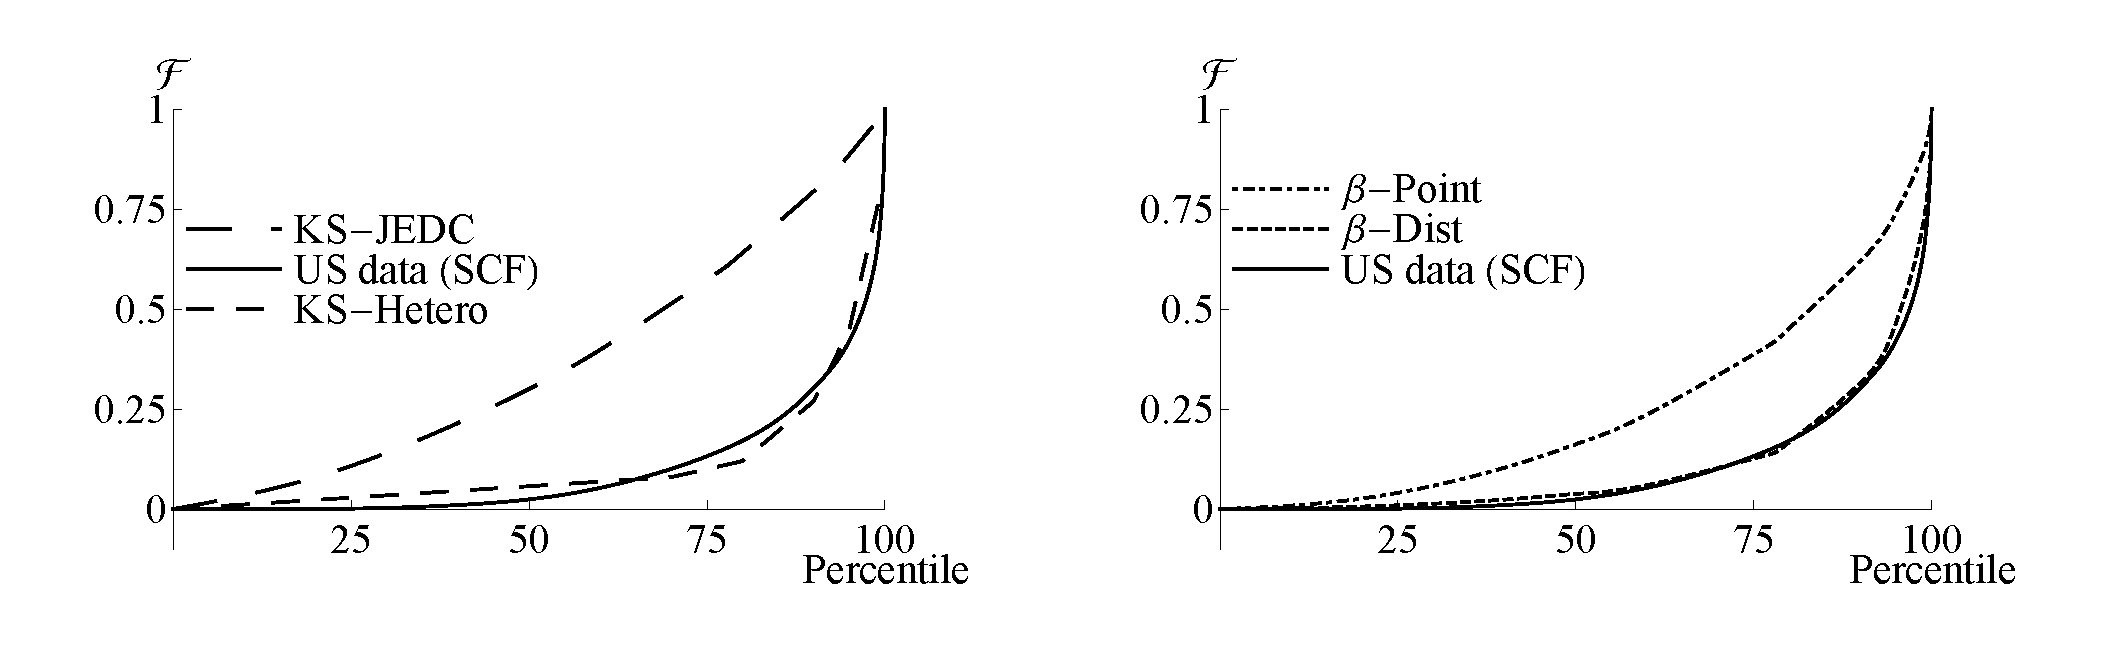
\includegraphics[width=1.00\textwidth]{../Figures/CumWLevSCFCastanedaAndDistSevenNoAggShockLRPlot}
% \CDCFig{CumWLevSCFCastanedaAndDistSevenNoAggShockTBPlot} % show two sub figures top and bottom
\footnotesize Notes: The solid curve shows the distribution of net worth in the 2004 \emph{Survey of Consumer Finances}. KS-Hetero is from \citet{ksHetero}.
\end{figure}

However, the wealth heterogeneity in the $\Discount$-Point model essentially just replicates heterogeneity in permanent income (which accounts for most of the heterogeneity in total income); for example the Gini coefficient for permanent income measured in the \emph{Survey of Consumer Finances} of roughly 0.5 is similar to that for wealth generated in the $\Discount$-Point model.  Since the empirical distribution of wealth (which has the Gini coefficient of around 0.8) is considerably more unequal than the distribution of income (or permanent income), the setup only captures part of the wealth heterogeneity in the data, especially at the top.


\begin{comment}

  Comparison of the relevant values in Table~\ref{table:ParamsAll} makes clear that the  aggregate shocks are in terms of variance 100 times smaller than the idiosyncratic shocks. Consequently, it is no surprise that the key quantitative results of our analysis so far generalize to the framework which includes realistically calibrated aggregate uncertainty. In particular, the two rightmost columns of Table~\ref{table:MPCall} with the MPC breakdowns from the $\Discount$-Dist models with aggregate shocks closely mirror columns~2~and~3, in which these shocks are shut down.
  For example, in the net worth case, the aggregate MPC for the model calibrated to the distribution of the net worth is $
  \input ../Code/Mathematica/Results/MPCDistSevenWithAggPermShocks.tex
  $, while that for the liquid financial and retirement assets case remains much higher at
  $
  \input ../Code/Mathematica/Results/MPCDistSevenWithAggPermShocksLiqFinPlsRet.tex
  $.

  % \footnote{As in the net worth case, parameter value are estimated with aggregate shocks turned off
  % ($(\grave{\Discount}, \nabla)=(
  % \input ../Code/Mathematica/Results/BetamiddleLiqFinPlsRet.tex
  % ,
  % \input ../Code/Mathematica/Results/NablaLiqFinPlsRet.tex
  % )$).}

\end{comment}

\subsection{Heterogeneous Impatience: The `$\Discount$-Dist' Model}

Because we want a modeling framework that matches the fact
that wealth inequality substantially exceeds income inequality, we
need to introduce an additional source of heterogeneity (beyond heterogeneity in permanent and transitory income).  We accomplish this
by introducing heterogeneity in impatience.  Each household is now assumed to
have an idiosyncratic (but fixed) time preference factor.  We think of
this assumption as reflecting not only actual variation in pure rates
of time preference across people, but also as reflecting other
differences (in age, income growth expectations, investment
opportunities, tax schedules, risk aversion, and other variables) that
are not explicitly incorporated into the model.

To be more concrete, take the example of age.  A robust pattern in
most countries is that income grows much faster for young people than
for older people.  Our ``death-modified growth impatience condition'' \eqref{eq:GIC}
captures the intuition that people facing faster income growth tend to
act, financially, in a more `impatient' fashion than those facing
lower growth.  So we should expect young people to have lower target
wealth-to-income ratios than older people.  Thus, what we are
capturing by allowing heterogeneity in time preference factors is
probably also some portion of the difference in behavior that (in
truth) reflects differences in age instead of in pure time preference
factors.  Some of what we achieve by allowing heterogeneity in
$\Discount$ could alternatively be introduced into the model if we had
a more complex specification of the life cycle that allowed for
different income growth rates for households of different ages. We make this point quantitatively
in section~\ref{sec:LCM} below, which solves the `$\Discount$-Dist' model in a realistic life cycle framework.

One way of gauging a model's predictions for wealth inequality is to
ask how well it is able to match the proportion of total net worth held
by the wealthiest $20$, $40$, $60$, and $80$ percent of the population.
We follow other papers (in particular \citet{castaneda}) in matching
these statistics.\footnote{\citet{castaneda} targeted various wealth and income
  distribution statistics, including net worth held by the top $1$, $5$, $10$, $20$,
  $40$, $60$, $80$ percent, and the Gini coefficient.}
% The footnote listed all the (wealth) statistics Castaneda matched. Note that they are matching various income statistics as well.

Our specific approach is to replace the assumption that all households have the same time
preference factor with an assumption that, for some dispersion $\nabla$, time
preference factors are distributed uniformly in the population between
$\grave{\Discount}-\nabla$ and $\grave{\Discount}+\nabla$ (for this reason, the model is referred to as the `$\Discount$-Dist' model).  Then,
using simulations, we search for the values of $\grave{\Discount}$ and
$\nabla$ for which the model best matches the fraction of net worth held by the top $20$, $40$, $60$, and $80$ percent of the population, while at the same time matching
the aggregate capital-to-output ratio from the perfect foresight
model. Specifically, defining $w_{i}$ and $\omega _{i}$ as the proportion of total aggregate net worth held by the top $i$ percent in our model and in the data, respectively, we solve the following minimization problem:
\begin{equation}
  \{\grave{\Discount}, \nabla\}= \underset{\{{\Discount}, \nabla\}}{\text{argmin} }\Big(\sum_\text{$i=20$, $40$, $60$, $80$}
  \big(w_{i}({\Discount}, \nabla)-\omega _{i}\big)^{2}\Big)^{1/2} \label{eq:MinimizationProb}
\end{equation}
subject to the constraint that the aggregate wealth (net worth)-to-output ratio in the model matches the aggregate
capital-to-output ratio from the perfect foresight model ($\KLev_{PF}/\YLev_{PF}$):\footnote{In estimating these parameter values, we approximate the uniform distribution with the following seven points (each with the mass of $1/7$): $\{\grave{\Discount}-3\nabla/3.5$, $\grave{\Discount}-2\nabla/3.5$, $\grave{\Discount}-\nabla/3.5$, $\grave{\Discount}$, $\grave{\Discount}+\nabla/3.5$, $\grave{\Discount}+2\nabla/3.5$, $\grave{\Discount}+3\nabla/3.5\}$. Increasing the number of points further does not notably change the results below. When solving the problem \eqref{eq:MinimizationProb}--\eqref{eq:pfConstraint} for the FBS specification we shut down the aggregate shocks (practically, this does not affect the estimates given their small size).
  \label{foot:uniApprox}}
\begin{eqnarray}
  \KLev/\YLev & = & \KLev_{PF}/\YLev_{PF}.  \label{eq:pfConstraint}
\end{eqnarray}
The solution to this problem is $\{\grave{\Discount}, \nabla\}=\{
\input ../Code/Mathematica/Results/Betamiddle.tex
,
\input ../Code/Mathematica/Results/Nabla.tex
\}$, so that the discount factors are evenly spread roughly between 0.98 and 0.99.\footnote{With these estimates, even the most patient consumers with $\Discount=\grave{\Discount}+3\nabla/3.5$ (see footnote~\ref{foot:uniApprox}) satisfy the death-modified `Growth Impatience Condition' of \eqref{eq:GIC} (a sufficient condition for stationarity of the wealth distribution), derived in Appendix C of \citet{cstKS} (ECB working paper). \label{foot:DMGIC} } We call the optimal value of the objective function \eqref{eq:MinimizationProb} the `Lorenz distance' and use it as a measure of fit of the models.

The introduction of even such a relatively modest amount of time
preference heterogeneity sharply improves the model's fit to the targeted
proportions of wealth holdings, bringing it reasonably in line with the data (Figure~\ref{CumWLevSCFCastanedaAndDistSevenNoAggShockPlot}).%
\footnote{The Lorenz distance falls from almost 40 for the $\Discount$-Dist model to just above 2 for the $\Discount$-Dist model; see Table~\ref{table:MPCall}.}
The
ability of the model to match the targeted moments does not, of
course, constitute a formal test, except in the loose sense that a
model with such strong structure might have been unable to get nearly
so close to four target wealth points with only one free
parameter.\footnote{Because the constraint \eqref{eq:pfConstraint} effectively pins down the discount factor $\grave{\Discount}$
  estimated in the minimization problem \eqref{eq:MinimizationProb},
  only the dispersion $\nabla$ works to match the four wealth target points.} But the model also sharply improves the fit to locations in
the wealth distribution that were not explicitly targeted; for
example, the net worth shares of the top 10 percent and the top 1
percent are also shown in the figure, and the model performs
reasonably well in matching them.%
\footnote{%
  We have examined the results for alternative calibrations of $\CRRA$ (section~\ref{sec:Sensitivity}); unsurprisingly, for larger calibrations of $\CRRA$, $\nabla$ is larger.  For example, for $\CRRA=2$, $\nabla$ is a bit more than twice as large.  However, implications for the MPC are roughly similar.
}

Of course, \citet{ksHeteroPort,ksHetero} were well aware that their baseline model
provides a poor match to the wealth distribution.  In response, they
examined whether inclusion of a form of discount rate heterogeneity
could improve the model's match to the data.  Specifically, they
assumed that the discount factor takes one of the three values
$\{0.9858, 0.9894, 0.9930\}$, and that agents anticipate that
their discount factor might change between these values according to a
Markov process. As they showed, the model with this simple form of
heterogeneity did improve the model's ability to match the wealth
holdings of the top percentiles (see Figure~\ref{CumWLevSCFCastanedaAndDistSevenNoAggShockPlot}).\footnote{Indeed, their results show that their model of heterogeneity went a bit too far: it concentrated almost all of the net worth in the top 20 percent of the population.  By comparison, our model $\Discount$-Dist does a notably better job matching the data across the entire span of wealth percentiles.}

The reader might wonder why we do not simply adopt the KS
specification of preference heterogeneity, rather than
introducing our own novel (though simple) form of heterogeneity.  The
principal answer is that our purpose here is to define a method of
explicitly matching the model to the data via statistical estimation
of a parameter of the distribution of heterogeneity: we let the data
speak flexibly about the extent of the preference heterogeneity
required in the model.  Krusell and Smith were not estimating
a distribution in this manner; estimation of their framework would have required
searching for more than one parameter, and possibly as many as three or four.  Indeed, had they intended
to estimate parameters, they might have chosen
a method more like ours.  Second, having
introduced finite horizons in order to yield an ergodic distribution
of permanent income, it would be peculiar to layer on top of the
stochastic death probability a stochastic probability of changing
one's time preference factor within the lifetime.\footnote{Krusell and Smith
  motivated their differing time preference factors as reflecting
  different preferences of alternating generations of a dynasty, but
  with our finite horizons assumption we have eliminated the dynastic
  interpretation of the model.}${}^,$\footnote{\cite{kruegerMitmanPerri:handbookMacro} use our specification of preference heterogeneity to investigate the dynamics of their model economy during the Great Recession.}
Third, our results below show that the Krusell and Smith
specification of discount rate heterogeneity implies a substantially lower aggregate MPC than our $\Discount$-Dist model.  Having said all of this, the common
point across the two papers is that a key requirement to make the
model fit the wealth data is a form of heterogeneity that leads different
households to have different target levels of wealth.

\section{The MPC in the Perpetual Youth Model} \label{sec:MPC}


Having constructed a model with a realistic household income process which is able to reproduce steady-state wealth heterogeneity in the data, we now turn on aggregate shocks and investigate the model's implications about relevant macroeconomic questions.
In particular, we ask whether a
model that manages to match the distribution of wealth has similar, or
different, implications from the KS-JEDC or representative agent
models for the reaction of aggregate consumption to an economic
`stimulus' payment.

Specifically, we pose the question as follows.  The economy has been
in its steady-state equilibrium leading up to date $t$.  Before the
consumption decision is made in that period, the government announces
the following plan: effective immediately, every household in the
economy will receive a one-off `stimulus check' worth some modest
amount (financed by a tax on unborn future
generations).\footnote{This financing scheme, along with the lack of a
  bequest motive, eliminates any Ricardian offset that might otherwise
  occur.} Our question is: \emph{By how much will aggregate consumption increase?}

\subsection{Matching Net Worth}

In theory, the distribution of wealth across recipients of the stimulus checks has important implications for aggregate MPC out
of transitory shocks to income. To see why, the solid line of Figure~\ref{CFuncDistSevenPointPermAndHistNetWorthPlotFedQuarterly} plots our $\Discount$-Point model's individual
consumption function using the FBS aggregate income process, with the
horizontal axis being cash on hand normalized by the level of
(quarterly) permanent income. Because the households with less normalized cash have higher MPCs, the average MPC is higher when a larger fraction of households has less (normalized) cash on hand.

\begin{figure}
    \caption{Empirical Wealth Distribution and Consumption Functions of the
      $\Discount$-Point and $\Discount$-Dist Models}
    \label{CFuncDistSevenPointPermAndHistNetWorthPlotFedQuarterly}
  \begin{center}
    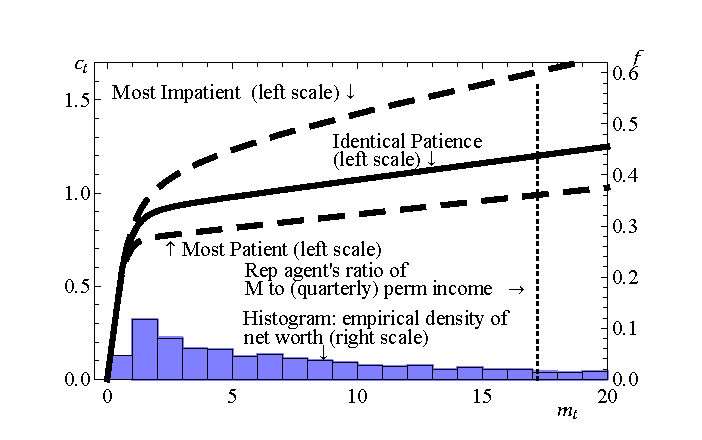
\includegraphics{./Figures/CFuncDistSevenPointPermAndHistNetWorthPlotFedQuarterly}
  \end{center}
    \footnotesize Notes: The solid curve shows the consumption function
    for $\Discount$-Point model, and the dashed curves show the consumption functions
    for the most patient and the least patient consumers for
    $\Discount$-Dist model (under the FBS aggregate process). The histogram shows the empirical distribution of
    net worth ($\mRat_{t}$) in the \emph{Survey of Consumer Finances} of 2004.
\end{figure}

There are many more households with little wealth in our $\Discount$-Point model than in the KS-JEDC model, as illustrated by comparison of the dash-dotted and the long-dashing lines in Figure~\ref{CumWLevSCFCastanedaAndDistSevenNoAggShockPlot}. The greater concentration of wealth at the bottom in the $\Discount$-Point model, which mirrors the data (see the histogram in Figure~\ref{CFuncDistSevenPointPermAndHistNetWorthPlotFedQuarterly}), should produce a higher average MPC, given the concave consumption function.

Indeed, the average MPC out of the transitory income (`stimulus check') in our $\Discount$-Point model is $ \input ../Code/Mathematica/Results/MPCPointWithAggShock.tex $ in annual terms (third column of Table~\ref{table:MPCall}),\footnote{The casual usage of the term `the MPC' refers to annual MPC given by $1-(1-\text{quarterly MPC})^4$ (recall again that the models in this paper are calibrated quarterly).  We make this choice because existing influential empirical studies (e.g., \citet{souleles:taxrefunds}; \citet{jpsTax}) estimate longer-term MPCs for the amount of extra spending that has occurred over the course of \emph{a year or 9 months} in response to a one unit increase in resources.}  about double the value in the KS-JEDC model $( \input ../Code/Mathematica/Results/MPCKSWithAggShock.tex )$ (first column of the table) or the perfect foresight partial equilibrium model with parameters matching our baseline calibration (0.04). Our $\Discount$-Dist model (fourth column of the table) produces an even higher average MPC $( \input ../Code/Mathematica/Results/MPCDistSevenWithAggShock.tex )$, since in the $\Discount$-Dist model there are more households who possess less wealth, are more impatient, and have higher MPCs (Figure~\ref{CumWLevSCFCastanedaAndDistSevenNoAggShockPlot} and dashed lines in Figure~\ref{CFuncDistSevenPointPermAndHistNetWorthPlotFedQuarterly}). However, this is still at best only at the lower bound of empirical MPC estimates, which are typically between $0.2$--$0.6$ or even higher (see Table~\ref{table:mpcLit}).%
\footnote{The MPCs calculated in Table~\ref{table:MPCall} are `theoretical', i.e., based on the slope of the consumption function. Alternatively, we have also calculated the following `discrete' MPCs based on an increase in spending over the next four quarters after the household received an unexpected \$ 1,000 extra in income. The implied MPCs for such calculation are slightly lower than the ones we report, e.g., for the aggregate MPC in the perpetual youth $\Discount$-Dist model we get a value of \input ../Code/Mathematica/Results/MPCAltDistSevenWithAggPermShocks.tex (instead of \input ../Code/Mathematica/Results/MPCDistSevenWithAggPermShocks.tex reported in column~6 of Table~\ref{table:MPCall}).}

\begin{figure}
  \caption{Consumption Functions of  $\Discount$-Dist and KS-Hetero Models and the Distribution of Cash on Hand}
  \label{CFuncKSHeteroAndDistSevenAndHistDataKSHeteroPlot}
  \begin{center}
    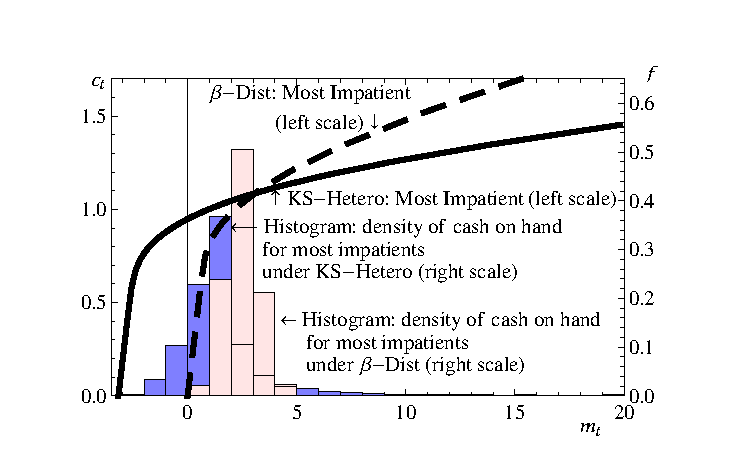
\includegraphics{./Figures/CFuncKSHeteroAndDistSevenAndHistDataKSHeteroPlot}
  \end{center}
    {\footnotesize Notes: The dashed curve and the solid curve show the consumption functions for the most impatient consumers in $\Discount$-Dist model and the KS-Hetero model under the KS aggregate process, respectively. The consumption functions are for employed consumers in the good aggregate state. The pink (light grey) and blue (dark grey) histograms show the distributions of cash on hand for the most impatient consumers generated by $\Discount$-Dist model and the KS-Hetero model, respectively.}
\end{figure}

Column~3 reports that the Krusell--Smith model with heterogeneous discount rates, `KS-Hetero' has very different implications about marginal propensities than $\Discount$-Dist model.  While both models match the empirical wealth distribution, the KS-Hetero model generates a much lower aggregate MPC: 0.09. Figure~\ref{CFuncKSHeteroAndDistSevenAndHistDataKSHeteroPlot} shows the reason for this discrepancy: in the KS-Hetero model, a large fraction of even the most impatient households stay in the region where the consumption function is flat and the MPC is low (see the solid line and the blue (dark grey) histogram). In addition, the heterogeneity in MPCs across wealth--income ratios is substantially lower than in the $\Discount$-Dist model: In the KS-Hetero model households in the bottom 20 \%\ have MPCs of around 0.2, while in the $\Discount$-Dist model almost 0.5.
% \jbemph{Need to discuss why MPCs are low in KS-Hetero.}

To further understand the role of various components of the $\Discount$-Dist model and the differences in the mechanics of the $\Discount$-Dist and the KS-Hetero models we have turned off the permanent $\pshk$ and transitory $\tShkEmp$ income shocks, and the borrowing constraint. We find that turning off transitory shocks does not noticeably affect the MPC. Turning off the permanent shocks \emph{and} allowing for borrowing up to the half of annual permanent income, $\wEndRat_{t\iSub}\geq-2$ (like in the KS-Hetero model) reduces the aggregate MPC from 0.21 to 0.14, each of these two items contributing roughly the same to the decline.\footnote{A setup without the shocks $\pshk$ and $\tShkEmp$ is similar to the KS-Hetero model in that it replicates their idiosyncratic income process.  Such setup with a less strict borrowing constraint (like in KS-Hetero) implies an aggregate MPC of 0.14.  The remaining differences from KS-Hetero are the specification of aggregate shocks and the nature of $\Discount$ heterogeneity.  As columns~4 and 6 in Table~\ref{table:MPCall} show that the aggregate MPC is similar under the FBS or KS aggregate process (0.21 vs.\ 0.23), we believe the residual difference in MPCs is mostly or entirely accounted for by the vastly different assumptions about the distribution of $\Discount$.  While the lowest, middle, and highest discrete values of $\Discount$ in our $\Discount$-Dist specification are \textit{very} close to the three KS $\Discount$ values, $(0.9858,0.9894,0.9930)$, about 29\% of our simulated agents have an intermediate $\Discount$ between the lowest and central types; the corresponding percentiles of $\Discount$ in the KS-Hetero model (as well as the 4\% below that) all have $\Discount=0.9894$.  As the average MPC is convex in $\Discount$, this relative dispersion of the central mass results in an increased MPC in $\Discount$-Dist relative to KS-Hetero even when idiosyncratic income shocks are shut down and borrowing is allowed.  These results are reported in our online appendix.}


% \begin{sidewaystable}
%   \input ../Tables/MPCall
% \end{sidewaystable}

\begin{sidewaystable}
  \caption{Average (Aggregate) Marginal Propensity to Consume in Annual Terms}
  \label{table:MPCall}
  \begin{minipage}{\textwidth}
    \input ../Tables/MPCall_LCM
    {\footnotesize Notes: Annual MPC is calculated by $1-(1-$\text{quarterly MPC}$)^{4}$.  ``Liquid Assets'' refers to liquid financial plus retirement assets. ${}^\ddagger$: Discount factors are uniformly distributed over the interval $[\grave{\Discount}-\nabla,\grave{\Discount}+\nabla]$.  ${}^\star$: The Lorenz distance is defined as: $\underset{\{{\beta}, \nabla\}}{\min} \Big(\sum_{i=20, 40, 60, 80}\big(w_{i}({\beta},\nabla)-\omega_{i}\big)^{2}\Big)^{1/2}$ where $w_{i}$ and $\omega_{i}$ are the proportions of total aggregate net worth held by the top $i$ percent in the model and in the data, respectively.  }
  \end{minipage}
\end{sidewaystable}

% Old version with \text breaks TeX4HT: {\footnotesize Notes: Annual MPC is calculated by $1-(1-$\text{quarterly MPC}$)^{4}$. ``Liquid Assets'' refers to liquid financial plus retirement assets. ${}^\ddagger$: Discount factors are uniformly distributed over the interval $[\grave{\Discount}-\nabla,\grave{\Discount}+\nabla]$. ${}^\star$: The Lorenz distance is defined as: $\underset{\{{\beta}, \nabla\}}{\min}\Big(\sum_\text{$i=20$, $40$, $60$, $80$} \big(w_{i}({\beta},\nabla)-\omega_{i}\big)^{2}\Big)^{1/2}$, where $w_{i}$ and $\omega_{i}$ are the proportions of total aggregate net worth held by the top $i$ percent in the model and in the data, respectively.}

% Excised because Tex4Ht balks on blank lines in figs and tables
% $^{\ddagger}:$ $\grave{\Discount}=
% \input ../Code/Mathematica/Results/Beta.tex
% $.
% $^{\star}:$ $(\grave{\Discount}, \nabla)=(
% \input ../Code/Mathematica/Results/Betamiddle.tex
% ,
% \input ../Code/Mathematica/Results/nabla.tex
% )$, which implies $\{\grave{\Discount}-\nabla, \grave{\Discount}+\nabla\}=\{
% \input ../Code/Mathematica/Results/BetaLow.tex
% ,
% \input ../Code/Mathematica/Results/BetaHigh.tex
% \}$.


The MPCs are unevenly distributed across households with different wealth--permanent income ratios, ranging from 0.06 for the fifth (wealth--permanent income ratio) quintile to 0.48 for the first quintile, reflecting both the strong nonlinearity of the consumption function (in Figure~\ref{CFuncDistSevenPointPermAndHistNetWorthPlotFedQuarterly}) and preference type ``sorting'' as more patient households have a lower MPC at every wealth ratio and thus have a higher target ratio. Such heterogeneity in the MPC has previously been estimated in several empirical papers (at least to the extent that data are informative about differences in propensities across households).\footnote{%
  See  \citet{bppInequality}, \citet{brodaParker:stimulus2008}, \citet{leth-petersen:liquidity}, \citet{jappelliPistaferri_FPMPC}, \citet{jpsTax}, \citet{aslCredit} and  \citet{bps:familyLaborS}}

The income gradient of the MPC (bottom panel of Table~\ref{table:MPCall}) is much shallower than for the wealth ratio-- only households in the bottom income quintile have considerably higher MPCs (0.35 with KS aggregate shocks) than the rest (around 0.20).  This occurs because low income can result from either low transitory or permanent shocks; the former tends to increase the MPC while the latter decreases it.  In the $\Discount$-Point model, where almost all households are well insured, the income-MPC gradient is nearly flat, with a slight inverted U-shape.  In the $\Discount$-Dist model, about 75\% of households are more impatient than in $\Discount$-Point, and many have a fairly low target wealth ratio; bound by the credit constraint $\wEndRat_t \geq 0$, these households' wealth-to-income ratios are thus more sensitive to low transitory shocks than low permanent shocks, and thus low income is associated with a higher MPC on average.\footnote{The income-MPC gradient in the $\Discount$-Dist columns is the \textit{average} across the seven $\Discount$-types.  Though it is flat (or inverted U-shaped) for the more patient types, it is much steeper for less patient types.  Note that the gradient is steeper with KS shocks than with FBS shocks, because the former has a greater proportion of less patient households.}

\cite{kaplanViolanteWeidner_wealthyH2M} estimate that roughly a third of U.S. households are hand-to-mouth (in that they spend all their income in every pay-period). Of these households, roughly two thirds are wealthy---they own an illiquid asset---and the rest are poor. Because a state variable in our model is the ratio of wealth to permanent income, it can well be that households with low wealth--permanent income ratios own relatively high wealth (if their permanent income is high). In fact, a tabulation of the one third of households with the highest MPCs in the $\Discount$-Dist model reveals that these households have quite diverse wealth holdings: half of them are in the bottom wealth quintile, one-third are in the second quintile and about 15 percent are in the third quintile.

Comparison of the fourth and sixth columns of Table~\ref{table:MPCall} makes it clear that for the purpose of
backing out the aggregate MPC, the particular form of the aggregate
income process is not essential; both in qualitative and in
quantitative terms the aggregate MPC and its breakdowns for the KS and
the FBS aggregate income specification lie close to each other.  This
finding is in line with a large literature sparked by
\citet{lucasBusinessCycles} about the modest welfare cost of the
aggregate fluctuations associated with business cycles and with the
calibration of Table~\ref{table:ParamsAll}, in which variance of
aggregate shocks is roughly two orders of magnitude smaller than
variance of idiosyncratic shocks.\footnote{Of course, if one consequence of
  business cycles is to increase the magnitude of idiosyncratic shocks,
  as suggested for example by \cite{mcKayPapp:wageRiskOverBC}, \cite{gosCyclical} and \cite{Blundell:2013tm}, the costs of business cycles could be much larger than in traditional calculations that
  examine only the consequences of aggregate shocks.}


\subsection{Matching Liquid Assets}
Thus far, we have been using total household net worth as our measure
of wealth.  Implicitly, this assumes that all of the household's debt
and asset positions are perfectly liquid and that, say, a household
with home equity of \$50,000 and bank balances of \$2,000 (and no
other balance sheet items) will behave in every respect similarly to a
household with home equity of \$10,000 and bank balances of \$42,000.
This seems implausible.  The home equity is more illiquid (tapping it
requires, at the very least, obtaining a home equity line of credit,
with the attendant inconvenience and expense of appraisal of the house
and some paperwork).

\citet{otsukaIlliquid} formally analyzes the optimization problem of
a consumer with a FBS income process who can invest in an illiquid but
higher-return asset (think housing), or a liquid but lower-return
asset (cash), and shows, unsurprisingly, that the annual marginal propensity
to consume out of shocks to liquid assets is higher than the MPC out
of shocks to illiquid assets.  Her results would presumably be even
stronger if she had permitted households to hold much of their wealth in illiquid forms (housing,
pension savings), for example, as a mechanism to overcome self-control problems
(see \citet{laibson:goldeneggs} and many others).\footnote{Indeed, using a model with both a low-return liquid asset and a high-return illiquid asset, \citet{kvStim} have replicated high MPCs observed in the data.}  % Alternatively, \citet{thalerMental} and others have argued that households construct `mental accounts' corresponding to different kinds of assets and have distinctly different behaviors (including different MPCs) with respect to similar shocks to different accounts.

These considerations suggest that it may be more plausible, for
purposes of extracting predictions about the MPC out of stimulus
checks, to focus on matching the distribution of liquid financial and retirement assets across households. The inclusion of retirement assets is arguable, %\footnote{Results for more restrictive definitions of liquid assets are available upon request from the authors.}
but a case for inclusion can be made because in the U.S.\ retirement assets such as IRA's and 401(k)'s can be liquidated under a fairly clear rule (e.g., a penalty of $10$ percent of the balance liquidated).

% \begin{table}
%   \caption{Proportion of Wealth Held by Percentile (in Percent)}
%   \label{table:LiqFinPlsRetAssetDist}
%   \begin{minipage}{\textwidth}
%     \input ../Tables/LiqFinPlsRetAssetDist_2
%     \tablenotessize{Notes: The data source is the 2004 Survey of Consumer Finances.}
%   \end{minipage}
% \end{table}


\begin{figure}
  \caption{Empirical Distribution of Liquid Financial
    Assets${}+{}$Retirement Assets and Consumption Functions of
    $\Discount$-Dist Model}
  \label{CFuncDistSevenAndHistNetWorthLiqFinPlsRetPlot}
  \begin{center}
    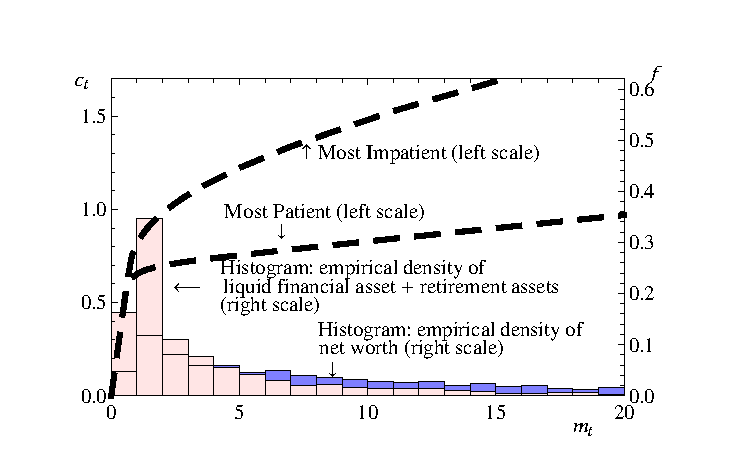
\includegraphics{./Figures/CFuncDistSevenAndHistNetWorthLiqFinPlsRetPlot}
  \end{center}
  \footnotesize Notes: The dashed curves show the consumption functions
  for the most patient and the least patient consumers for
  $\Discount$-Dist model under the KS aggregate process. The consumption functions are for employed consumers in the good aggregate state. The blue (dark grey) and pink (light grey)
  histograms show the empirical distributions of net worth and liquid
  financial and retirement assets, respectively, in the \emph{Survey of
    Consumer Finances} of 2004.
\end{figure}

When we ask the model to estimate the time preference factors that
allow it to best match the distribution of liquid financial and retirement assets (instead
of net worth),\footnote{We define liquid financial and retirement assets as the sum of transaction accounts (deposits),
  CDs, bonds, stocks, mutual funds, and retirement assets.  We take the same approach as before: we match
  the fraction of liquid financial and retirement assets held by the top $20$, $40$, $60$,
  and $80$ percent of the population (in the SCF 2004), while at the
  same time matching the aggregate liquid financial and retirement assets-to-income ratio (which is 6.6 in the SCF 2004).}
estimated parameter values are
$\{\grave{\Discount}, \nabla\}=\{
\input../Code/Mathematica/Results/BetamiddleWithAggShocksLiqFinPlsRet.tex ,
\input../Code/Mathematica/Results/NablaWithAggShocksLiqFinPlsRet.tex \}
$
under the KS aggregate income process and the average MPC is
$
\input../Code/Mathematica/Results/MPCDistSevenWithAggShockLiqFinPlsRet.tex
$ (fifth column of the table), which lies at the middle of the
range typically reported in the literature (see
Table~\ref{table:mpcLit}) and is considerably higher than when we
match the distribution of net worth.\footnote{When matching the distribution of liquid financial and retirement assets, we reduce the variance of permanent shocks $\sigma _{\pshk}^{2}$ to $0.01/4$ (from $0.01/(11/4)$ in Table~\ref{table:ParamsAll}) so that even the most patient consumers with  $\Discount=\grave{\Discount}+3\nabla/3.5$ satisfy the death-modified `Growth Impatience Condition' (see footnotes~\ref{foot:uniApprox} and \ref{foot:DMGIC}).} This reflects the fact that
matching the more skewed distribution of liquid financial and
retirement assets
(see
Figure~\ref{CFuncDistSevenAndHistNetWorthLiqFinPlsRetPlot}) requires
a wider distribution of the time preference factors, ranging between
0.94 and 0.98, which produces even more
households with little wealth.\footnote{The distribution of liquid financial and retirement assets is more concentrated close to zero than the distribution of net worth, e.g., the top 10 percent of households hold 75 percent of liquid assets and 70 percent of net worth.
  % The table also illustrates that both distributions did not change much over time.  It is well-known that in aggregate data from the Flow of Funds the ratio of net worth to annual income moves around quite a bit, between 4 and 6.5 in the past 40 years. However, note that these changes (i)  are in the flat region of the consumption function and, more important, (ii) are small relative to the cross-sectional dispersion in wealth.
}
The estimated distribution of discount factors lies below that obtained by matching net worth and is considerably more dispersed because of substantially lower median and more unevenly distributed liquid financial and retirement assets (compared to net worth).\footnote{Our value of the survival probability $\PLives=1 -0.00625$ implies that 8 percent of households are older than 100 years. To keep the model consistent we keep them in the economy.  However, the results essentially do not change---under the FBS aggregate shocks, the aggregate MPC is
  $
  \input ../Code/Mathematica/Results/MPCDistSevenWithAggPermShocksLiqFinPlsRetDeathFrAge.tex $
  instead of
  $
  \input ../Code/Mathematica/Results/MPCDistSevenWithAggPermShocksLiqFinPlsRet.tex $---if we alternatively replace the 100-year-olds with newborns (assuming they do not anticipate being replaced). This is reasonable given the small number of such households and given that the consumption function is almost linear at high levels of wealth.
}

\begin{figure}
  \begin{center}
    \caption{Distribution of MPCs Across Households}
    \label{MPCdist}
    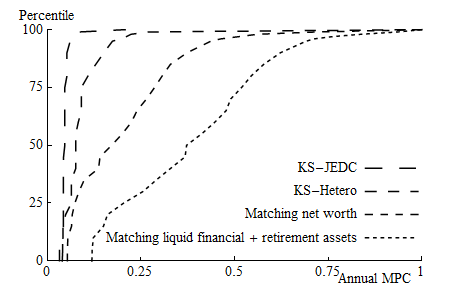
\includegraphics{./Figures/DistributionsMPCsDistSevenAndKSKSAggShocksPlot}
  \end{center}
\end{figure}

Figure~\ref{MPCdist} shows the cumulative distribution functions of
MPCs for the KS-JEDC model and the $\Discount$-Dist models (under the KS aggregate income shocks) estimated to match, first, the empirical distribution of net worth and, alternatively, of liquid
financial and retirement assets.\footnote{We have also solved a version of the model
  that matches only ``very liquid assets'' (excluding retirement and other assets that might not be instantly accessible); as would be expected, that exercise produces an even higher average MPC.}  The figure illustrates that the MPCs for KS-JEDC model are concentrated tightly around 0.05, which sharply
contrasts with the results for the $\Discount$-Dist models. Because
the latter two models match the empirical wealth distribution, they
imply that a substantial fraction of consumers have very little
wealth.

Table~\ref{table:MPCall} illustrates the distribution of MPCs by wealth, income, and employment status. In contrast to the KS-JEDC model, and to a lesser extent also to the KS-Hetero model, the $\Discount$-Point and in particular $\Discount$-Dist models generate a wide distribution of marginal propensities.  Given the considerable concavity of the theoretical consumption function in the relevant region, these results indicate that the aggregate response to a stimulus program will depend greatly upon which households receive the stimulus payments.  Furthermore, unlike the results from the baseline KS-JEDC model or from a representative agent model, the results from these simulations are easily consistent with the empirical estimates of aggregate MPCs in Table~\ref{table:mpcLit} and the evidence that households with little liquid wealth and without high past income have high MPCs.\footnote{These studies include \citet{bppInequality}, \citet{brodaParker:stimulus2008}, \citet{leth-petersen:liquidity} and \citet{jappelliPistaferri_FPMPC}.}

\subsection{The MPC over the Business Cycle} \label{ss:BusinessCycle}

Because our models include FBS or KS aggregate shocks, we can investigate how the economy's
average MPC and its distribution across households varies over the business cycle. Table~\ref{table:MPCscenarios} reports
the results for the following experiments with the $\Discount$-Dist models calibrated to the net worth distribution (and compares them to the baseline results from Table~\ref{table:MPCall}). For the model with KS aggregate shocks, in which recessions/expansions can be defined as bad/good realizations of the aggregate state:
\begin{enumerate}
\item `Expansions vs.\ Recessions': $\ptyLev_{t}=1+\bigtriangleup ^{\ptyLev}$ vs.\ $\ptyLev_{t}=1-\bigtriangleup ^{\ptyLev}$.
\item `Entering Recession': Bad realization of the aggregate state directly preceded by a good one: $\ptyLev_{t}=1-\bigtriangleup ^{\ptyLev}$ for which $\ptyLev_{t-1}=1+\bigtriangleup ^{\ptyLev}$.
\end{enumerate}
For the model with FBS aggregate shocks, we consider large bad realizations of the aggregate shock:
\begin{enumerate}
\item `Large Bad Permanent Aggregate Shock': bottom 1 percent of the distribution in the permanent aggregate shock
\item `Large Bad Transitory Aggregate Shock': bottom 1 percent of the distribution in the transitory aggregate shock
\end{enumerate}

\begin{sidewaystable}
  \caption{Marginal Propensity to Consume over the Business Cycle}
  \label{table:MPCscenarios}
  \begin{minipage}{\textwidth}
    \input ../Tables/MPC_scenarios
    \tablenotessize{Notes: Annual MPC is calculated by $1-(1-$\text{quarterly MPC}$)^{4}$. The scenarios
      are calculated for the $\Discount$-Dist models calibrated to the net worth distribution. For the KS aggregate shocks, the results are obtained by running the simulation over 1,000 periods, and the scenarios are defined as (i) `Recessions/Expansions': bad/good realization of the aggregate state, $1-\bigtriangleup ^{\ptyLev}$/$1+\bigtriangleup ^{\ptyLev}$; (ii) `Entering Recession': bad realization of the aggregate state directly preceded by a good one: $\ptyLev_{t}=1-\bigtriangleup ^{\ptyLev}$ for which $\ptyLev_{t-1}=1+\bigtriangleup ^{\ptyLev}$. The `baseline' KS results are reproduced from column~4 of Table~\ref{table:MPCall}. For the FBS aggregate shocks, the results are averages over 1,000 simulations, and the scenarios are defined as (i) `Large Bad Permanent Aggregate Shock': bottom 1 percent of the distribution in the permanent aggregate shock; (ii) `Large Bad Transitory Aggregate Shock': bottom 1 percent of the distribution in the transitory aggregate shock. The `baseline' FBS results are reproduced from column~6 of Table~\ref{table:MPCall}.}
  \end{minipage}
\end{sidewaystable}

In the KS setup, the aggregate MPC is countercyclical, ranging between 0.22 in expansions and 0.25 in recessions. The key reason for this business cycle variation lies in the fact that aggregate shocks are correlated with idiosyncratic shocks. The movements in the aggregate MPC are driven by the inadequately insured households at the bottom of the distributions of wealth and income. MPCs for rich and employed households essentially do not change over the business cycle. The scenario `Entering Recession' documents that the length of the recession matters, so that initially the MPCs remain close to the baseline values, and increase only slowly as the recession persists.

In the FBS setup, the distribution of the MPC displays very little cyclical variation for both transitory and permanent aggregate shocks. This is because the precautionary behavior of households is driven essentially exclusively by idiosyncratic shocks, as these shocks are two orders of magnitude larger (in terms of variance) and because they are uncorrelated with aggregate shocks.

Of course, these results are obtained under the assumptions that the parameters and expectations in the models are constant, and that the wealth distribution is exogenous.   These assumptions are likely counterfactual in events like the Great Recession, during which objects such as expectations about the future income growth or the extent of uncertainty may well have changed.

As Figure~\ref{CFuncDistSevenPointPermAndHistNetWorthPlotFedQuarterly} suggests, the aggregate MPC in our models is a result of an (inter-related) interaction between two objects:  The  distribution of wealth and the consumption function(s). During the Great Recession, the distribution of net worth shifted very substantially downward.  Specifically, \cite{brickerEtAl:SCF2010} document that over the 2007--2010 period median net worth fell 38.8 percent (in real terms).%
\footnote{%
  The \emph{Survey of Consumer Finances} also documents that net worth decreased considerably relative to income; for example, the median net worth-to-income ratio declined from 8.5 in 2007 to 5.6 in 2010.
}
\emph{Ceteris paribus,} these dynamics resulted an increase in the aggregate MPC, as the fraction of wealth-poor, high-MPC households rose substantially.

It is also likely that the second object, the consumption function, changed as many of its determinants (such as the magnitude of income shocks%
\footnote{%
  See, e.g., \cite{gosCyclical} and \cite{Blundell:2013tm}, and the literature on the `scarring' effect of deep recessions on workers' lifetime income profiles.\\
  \cite{cstMPCxc} document that an increase in the variance of transitory income shocks makes the consumption function steeper close to the origin.
}) have not remained unaffected by the recession. And, of course, once parameters are allowed to vary, one needs to address the question about how households form expectations about these parameters. These factors make it quite complex to investigate adequately the numerous interactions potentially relevant for the dynamics of the MPC over the business cycle. Consequently, we leave the questions about the extent of cyclicality of the MPC in more complicated settings for future research.


\subsection{Sensitivity Analysis}\label{sec:Sensitivity}

\begin{figure}
  \caption{Sensitivity Analysis: Aggregate Marginal Propensity to Consume}
  \label{KappaSensitivity}
  \begin{center}
    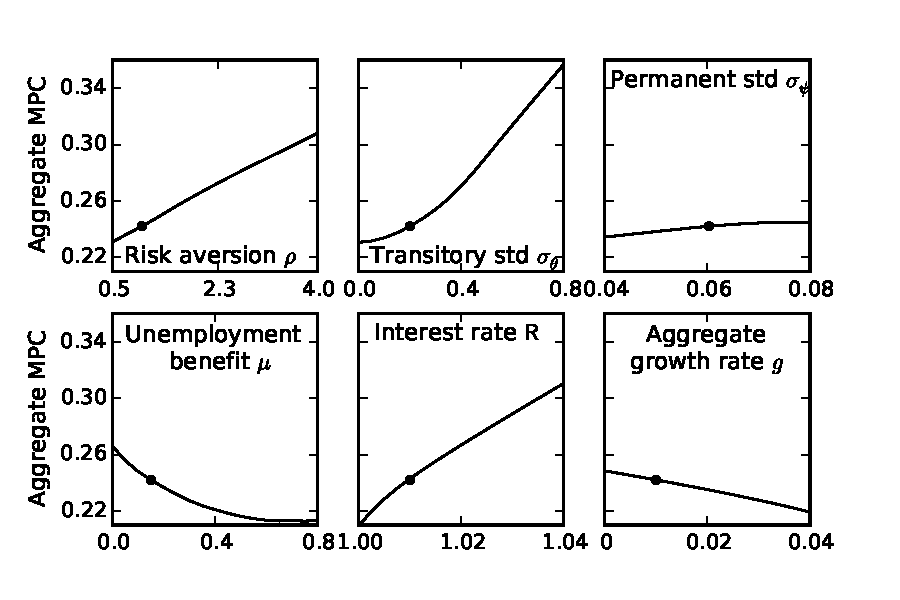
\includegraphics[scale=0.9]{./Figures/KappaSensitivity}
  \end{center}
\end{figure}

\begin{figure}
  \caption{Sensitivity Analysis: Distance Between Simulated \& Actual Lorenz Curves
  }
  \label{FitSensitivity}
  \begin{center}
    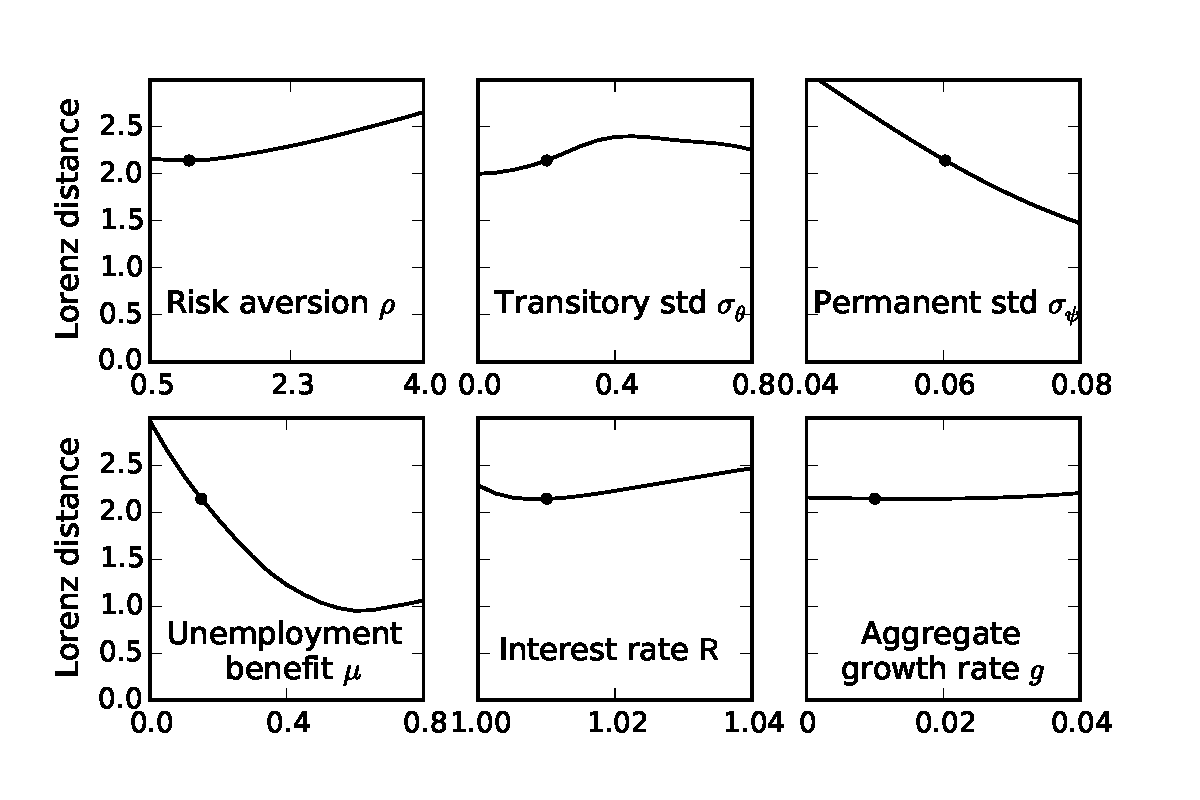
\includegraphics[scale=0.9]{./Figures/FitSensitivity}
  \end{center}
\end{figure}

\begin{figure}
  \caption{Sensitivity Analysis: Center of Discount Factor Distribution
  }
  \label{BetaSensitivity}
  \begin{center}
    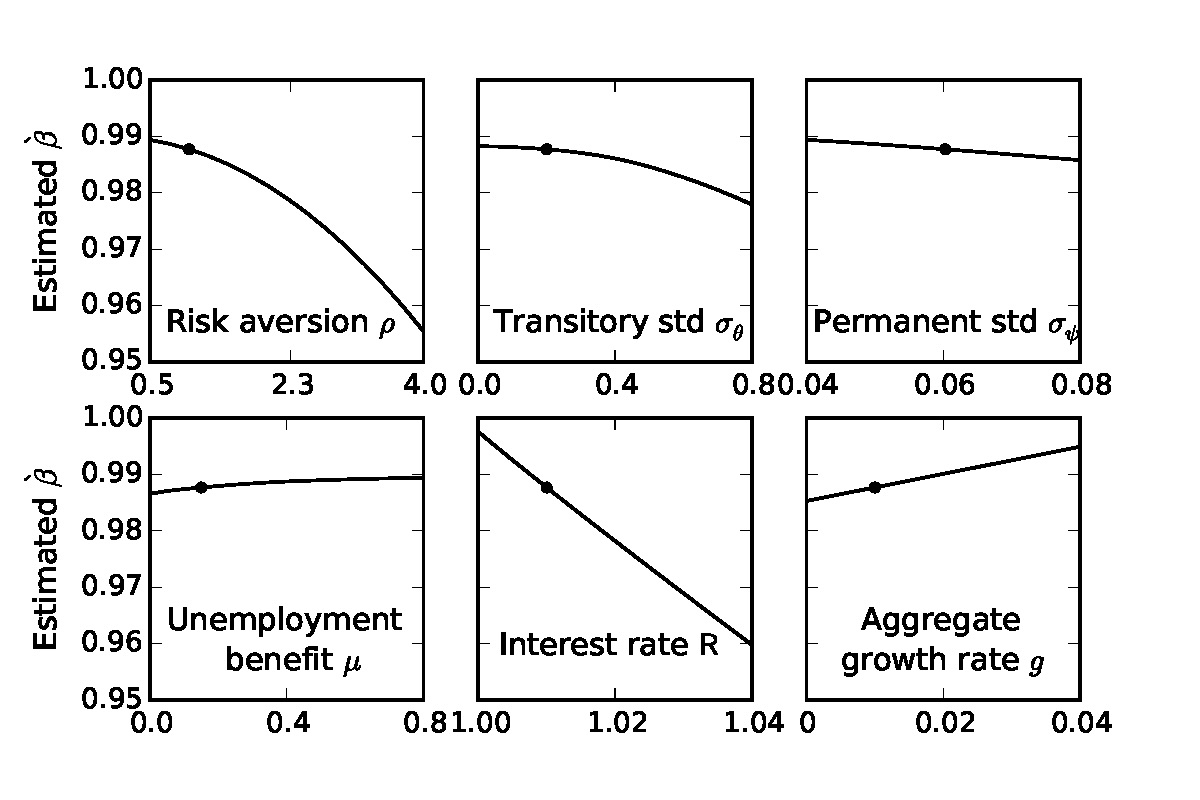
\includegraphics[scale=0.9]{./Figures/BetaSensitivity}
  \end{center}
\end{figure}

\begin{figure}
  \caption{Sensitivity Analysis: Width of Discount Factor Distribution
  }
  \label{NablaSensitivity}
  \begin{center}
    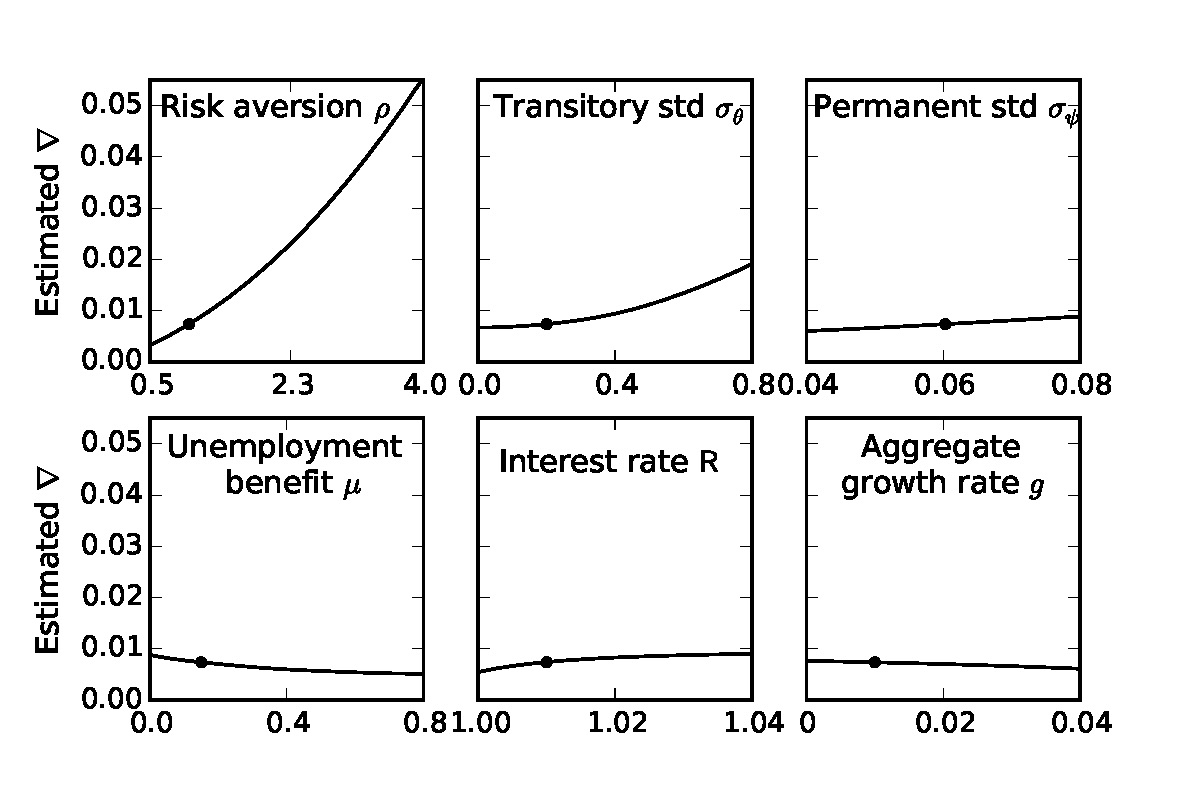
\includegraphics[scale=0.9]{./Figures/NablaSensitivity}
  \end{center}
\end{figure}

Because the literature does not agree on the precise values for some of our calibrated parameters, we want to understand the robustness of our results about the fit of the wealth distribution and about the MPC.
We investigated sensitivity to the calibrated parameters by re-estimating the $\Discount$-Dist model while varying one parameter at a time from its baseline value in Table~\ref{table:ParamsAll}; for example, we let the CRRA coefficient $\CRRA$ range between 0.5 and 4.  Figures~\ref{KappaSensitivity}--\ref{NablaSensitivity} show the results of the sensitivity analysis for six parameters: risk aversion $\CRRA$, transitory income shock standard deviation $\sigma_\theta$, permanent income shock standard deviation $\sigma_\psi$, unemployment benefit replacement rate $\mu$, gross interest factor $\mathsf{R}$, and the (annual) expected growth rate $g \equiv \Gamma^4 - 1$.\footnote{For this robustness exercise, we shut down aggregate shocks and set an exogenous $\mathsf{R}$.}  Overall, our main results are quite robust to alternative parameters, with the aggregate MPC consistently greater than 0.2 and a similar fit to the empirical wealth distribution.

The amount of discount factor heterogeneity needed to fit the Lorenz curve is nearly constant with respect to the calibrated parameters, as shown in Figure~\ref{NablaSensitivity}.  The only exceptions are when transitory shocks are much larger than most empirical estimates (three to four times the size of our baseline calibration) or when households are more risk averse.  In both cases, households are motivated to hold more precautionary wealth, and thus the model estimates that they have a lower average discount factor to fit the K/Y ratio and lower tail of the wealth distribution (in Figure~\ref{BetaSensitivity}); the width of the $\Discount$ distribution must thus be wider to generate households that hold large amounts of wealth because they nearly violate the Growth Impatience Condition \eqref{eq:GIC}.\footnote{The large estimated $\nabla$ for these parameterizations would be significantly tempered if we relaxed the credit constraint $\wEndRat_t \geq 0$, as the lower range of discount factors $\grave{\Discount} - \nabla$ would not need to be so low to generate households who hold slightly positive wealth.  Relaxing the credit constraint would also likely reduce the gradient in the MPC in Figure~\ref{KappaSensitivity}.}  With a larger proportion of impatient households, high $\CRRA$ and high $\sigma_\theta$ environments also imply a greater aggregate MPC (in Figure~\ref{KappaSensitivity}), reaching $0.28$ when $\rho=4$ and $0.33$ when $\sigma_\theta = 0.8$.

Varying the interest factor $\mathsf{R}$ has little effect on the estimated width $\nabla$, but a very large effect on the average discount factor $\grave{\Discount}$.  The interest and discount factors are very close substitutes in determining target wealth, and thus $\grave{\Discount}$ decreases at a slope of nearly $-1$ with respect to $\mathsf{R}$; the resulting impatient households have a higher MPC.  Among the remaining parameters, only higher unemployment benefits $\mu$ (moderately) lower the MPC as uncertainty is reduced.  The other considered parameters have little effect on the implied aggregate MPC, the fit of the wealth distribution,\footnote{Very low values of permanent income shock standard deviation $\sigma_\psi$ can lead to worse model fit, as permanent income dispersion does not contribute to wealth dispersion (as in the baseline KS model).} the estimated discount factor $\beta$ and its dispersion $\nabla$.  In total, we judge our main results to be quite robust.



\section{The MPC in a Life Cycle Model}\label{sec:LCM}

For ease of exposition and tractability of the aggregate shock processes, the models used in previous sections assume that households have unbounded horizons, with no difference between ``old'' and ``young'' agents.  Our qualitative results hold even when households are instead assumed to live out a finite life cycle, with more realistic assumptions about changes in the income process and mortality as the household ages.  This section discusses the assumptions used in an overlapping generations life cycle specification and presents analogous results corresponding to the analysis in section \ref{sec:MPC} by re-estimating the \Discount-Point and \Discount-Dist models.  In this environment, wealth heterogeneity emerges not only from shocks to permanent and transitory income and differences in discount factors, but also through demographic differences in age and education, via differential mortality and income growth expectations.  While these latter factors were abstracted into time preference heterogeneity in our benchmark model, here we model them explicitly to demonstrate the robustness of our results to the simplifying assumptions.

\subsection{Life Cycle of a Household}\label{sec:LifeCycle}

The economy consists of a continuum of expected utility maximizing households with a common CRRA utility function over consumption, $\uFunc(\bullet) = \bullet^{1-\CRRA}/(1-\CRRA)$; each household has a time discount factor $\Discount$.  A household enters the economy at time $t$ aged 24 years, endowed with an education level $e \in \{D,HS,C\}$ (for dropout, high school, and college, respectively), an initial permanent income level $\pLev_0$, and a stock of capital $\kLev_0$.  Each quarter, the household receives (after tax) income, chooses how much of their market resources to consume and how much to save, and then transitions to the next quarter by facing shocks to mortality and income.

The FBS income process of section~\ref{sec:PlausibleAggModel} translates into the life cycle framework as follows. A household receives a permanent shock to income when transitioning into period $t$, denoted by $\pshk_t$ (along with the age--education-specific average growth factor $\overline{\pshk}_{es}$), as well as an after tax transitory shock $\tshk_t$.  The life cycle variant of the income process can be summarized by:
\begin{eqnarray*}
  \yLev_t &=& \tshk_t \pLev_t = (1 - \tau)\theta_t \pLev_t,\\
  \pLev_t &=& \pshk_t \overline{\pshk}_{es} \pLev_{t-1}.
\end{eqnarray*}
Households that have already lived for $s$ periods have permanent shocks drawn from a lognormal distribution with mean 1 and variance $\sigma^2_{\pshk s}$, and transitory shocks drawn from a lognormal distribution with mean $1/\erate$ and variance $\sigma^2_{\theta s}$ with probability $\erate = (1 - \urate)$ and a degenerate distribution at $\mu$ with probability $\urate$.  The prospect of unemployment (at rate $\urate$) is a completely transitory event: unemployment in period $t$ has no effect on the probability of unemployment in period $t + 1$.  The non-zero transitory shock when unemployed represents a welfare benefit funded by income taxes, as discussed below.  When transitioning from one period to the next, a household with education $e$ that has already lived for $s$ periods faces a $\PDies_{es}$ probability of death.  In the main specification, the assets of a household that dies are completely taxed by the government to fund activities outside the model.\footnote{As a further robustness check, we also estimate versions in which the assets of the newly deceased are distributed to a random household, with varying preferences for bequests. In an online appendix we show that under a wide range of parameters governing preferences over bequests, both the overall aggregate marginal propensity to consume and its decompositions by wealth and income are little changed from the original specification.
}

The household's permanent income level will be factored out from the problem, so that the only state variable that affects the choice of optimal consumption is normalized market resources $\mRat_t$.  After this normalization, the household's budget transition functions can be described by:
\begin{eqnarray}
  \label{LifeCycleConstraint1}
  \aRat_t &=& \mRat_t - \cRat_t,\\
  \label{LifeCycleConstraint2}
  \kRat_{t+1} &=& \aRat_t/\pshk_{t+1},\\
  \label{LifeCycleConstraint3}
  \mRat_{t+1} &=& (\daleth +\rProd) \kRat_{t+1} + \tshk_{t+1},\\
  \label{LifeCycleConstraint4}
  \aRat_t &\geq& 0.
\end{eqnarray}
These transition constraints are identical to the perpetual youth model except that capital owned by surviving households does not grow with the inverse survival probability, and income is taxed at a marginal rate $\tau$ depending on the household's age and employment status.

Starting from some terminal age $\overline{s}$ at which $\PDies_{e\overline{s}} = 1$, a household's problem can be solved by backward induction until $s = 0$.  At age $\overline{s}$, the household will consume all market resources, generating a consumption function of $\cLev_{e\overline{s}}(\mLev_t,\pLev_t) = \mLev_t = \mRat_t \pLev_t$ and a value function of $V_{e\overline{s}}(\mLev_t,\pLev_t) = \uFunc(\mLev_t) = \pLev_t^{1-\CRRA} \uFunc(\mRat_t)$.  At any earlier age, the value function is recursively defined by:
\begin{equation}
  \label{eq:LifeCycleValue}
  V_{es}(\mLev_t,\pLev_t) = \max_{\cLev_t} \uFunc(\cLev_t) + \Discount \PLives_{es} \Ex_t \left[ V_{es+1}(\mLev_{t+1},\pLev_{t+1})\right] \text{ s.t. \eqref{LifeCycleConstraint1}--\eqref{LifeCycleConstraint4}}.
\end{equation}
To eliminate the permanent income level as a state variable, further define the normalized consumption function as $\cFunc_{es}(\mRat_t) = \cLev_{es}(\mLev_t,\pLev_t)/\pLev_t$ and the normalized value function as $\vFunc_{es}(\mRat_t) = V_{es}(\mLev_t,\pLev_t)/\pLev_t^{1-\CRRA}$.  Dividing \eqref{eq:LifeCycleValue} by $\pLev_t^{1-\CRRA}$, the problem is reduced to a single state dimension and can be expressed as:
\begin{eqnarray}\label{eq:LifeCycleValue1}
  \vFunc_{es}(\mRat_t) &=& \max_{\cRat_t} \uFunc(\cRat_t) + \Discount \PLives_{es} \Ex_t \left[\pshk_{t+1}^{1-\CRRA} \vFunc_{es+1}(\mRat_{t+1})\right] \text{ s.t. \eqref{LifeCycleConstraint1}--\eqref{LifeCycleConstraint4}},\\
  \cFunc_{es}(\mRat_t) &=& \arg\max_{\cRat_t} \uFunc(\cRat_t) + \Discount \PLives_{es} \Ex_t \left[\pshk_{t+1}^{1-\CRRA} \vFunc_{es+1}(\mRat_{t+1})\right] \text{ s.t. \eqref{LifeCycleConstraint1}--\eqref{LifeCycleConstraint4}}. \nonumber
\end{eqnarray}
A standard envelope condition applies in this model, so that $\vFunc_{es}^{\prime}(\mRat_t) = \uFunc^{\prime}(\cFunc_{es}(\mRat_t))$, and the first order condition for the solution to \eqref{eq:LifeCycleValue1} is:
\begin{equation}
  \cRat_t^{-\CRRA} = (\daleth +\rProd) \Discount \PLives \Ex_t \left[ (\pshk_{t+1} \cRat_{t+1})^{-\CRRA} \right].
\end{equation}
In this way, the value function need not be tracked or recorded during the solution process, as the age-dependent consumption functions are sufficient.\footnote{In practice, we use the method of endogenous gridpoints, as originally described in \cite{carrollEGM}, to discretize the state space and approximate consumption functions at each age and education level.}

\subsection{Macroeconomic Dynamics}

The analysis in section \ref{sec:MPC} demonstrated that while there is considerable variation in the marginal propensity to consume across income, wealth, and employment status, the MPC does not appreciably change depending on the structure of aggregate shocks to the economy nor to the current macroeconomic state.  Moreover, for reasons previously discussed, it is fairly difficult to account for macroeconomic state variables in an overlapping generations model.  Rather than expend significant energy on a feature that would yield little of interest, we do not model aggregate shocks in this section but instead focus on the effects of idiosyncratic shocks and household-level dynamics.  However, there are some additional macroeconomic features of the model that warrant discussion.

Unlike the perpetual youth model, the economy is now perpetually growing, with each new cohort larger than the last and ongoing technological progress.  The expected permanent income growth for a household $\overline{\pshk}_{es}$ comprises the household's own effective labor supply growth plus technological growth.  When aggregating wealth, the contribution of a household that has already lived for $s$ quarters is thus discounted by a factor of $(1 + \Gamma)^{-s}$ relative to the youngest cohort, where $\Gamma$ is the technological growth rate.  Moreover, older households were born into smaller cohorts relative to the newest generation, so our population weighting scheme scales their contribution by the population growth rate $N$.

As mentioned in section \ref{sec:LifeCycle}, households are subject to a tax rate of $\tau$ depending on their age and employment status.  Households are assumed to retire at age 65 (i.e.\ when $s = 164$), captured in the model with an expected permanent growth factor well below 1 at this age.\footnote{The drop in permanent income at retirement depends on the household's education: dropouts' income fall by 44\%, high school graduates by 56\%, and college graduates by 69\%.}  Income before retirement is earned through labor, while income after retirement is provided by a pay-as-you-go social security system funded by taxes on the employed.  The social security tax rate is calculated as the rate that balances outlays to retired households and tax revenues from the working population:
\begin{equation*}
  \tau_{SS} = \frac{\sum_{e \in \{D,HS,C\}} \Big[ \theta_e \overline{\pLev}_{e0} \sum_{t = 164}^{384} \big( ((1 + \Gamma)(1+N))^{-t} \prod_{s=0}^t ( \overline{\pshk}_{es} \PLives_{es} ) \big) \Big]}
  {\sum_{e \in \{D,HS,C\}} \Big[ \theta_e \overline{\pLev}_{e0} \sum_{t = 0}^{163} \big( ((1 + \Gamma)(1+N) )^{-t} \prod_{s=0}^t ( \overline{\pshk}_{es} \PLives_{es} ) \big) \Big]}.
\end{equation*}
Here, $\theta_e$ is the proportion of each new generation with education level $e$, and $\overline{\pLev}_{e0}$ is the average permanent income of that education type when they enter the economy at age 24.  Note that neither permanent nor transitory shocks are relevant, as they average to unity across a cohort.  The tax to fund unemployment benefits is simply the product of the unemployment rate and the benefit replacement rate: $\tau_U = \urate \mu$.  Employed households pay a total income tax rate of $\tau = \tau_{SS} + \tau_U$, while unemployed and retired households have $\tau = 0$.

\subsection{Calibration}

Calibrations of the distributional parameters are taken from related estimates in the literature.  Average permanent income growth rates $\overline{\pshk}_{es}$ are calculated using the same trajectories as in \cite{Cagetti} for those with less than a high school education, a high school degree, and four or more years of college.  The permanent and transitory shock variances are approximated from the results of \cite{SabelhausSong}, with extrapolation for ages 55--64.\footnote{We assume that $\sigma^2_{\pshk} = \sigma^2_{\theta} = 0$ in retirement, so there is no income risk.}  Households are assumed to retire at age 65, withdrawing from the labor force and only receiving income from a pay-as-you-go social security system financed by taxes on the working population.  Baseline mortality rates at each age are taken from the Social Security Administration's 2010 Actuarial Life Table,\footnote{Following the bulk of related literature, we use women's mortality rates to allow us to simulate households living past the husband's death.} then adjusted by education level using estimates by \cite{BrownLiebmanPollet} and converted to quarterly probabilities;\footnote{For ages 101--120, we use the adjustment for age 100, as this table does not extend to very late ages to which very few people live.} households die with certainty if they reach age 120.  The unemployment benefit $\mu$ is set to 0.15 to match \cite{Cagetti}, while the unemployment probability is $\urate = 7\%$, the average rate in the perpetual youth model.

We assume that the population grows at a rate of 1\% annually, while total factor productivity grows at a 1.5\% annual rate; these approximately match long run rates in the United States.  Educational attainment rates are set to be fairly consistent with U.S. educational rates over the past twenty years, and average initial permanent (quarterly) income at age 24 for each educational group are roughly calibrated to recent data.\footnote{Precision here is unimportant: after several years of simulation, the initial permanent income differences between types matters much less than their income growth trajectories and idiosyncratic shocks.}  Each simulated household is given an initial lognormal shock to permanent income with standard deviation 0.4, approximately matching the total variance of income among young households in the SCF 2004 data.  Households begin with a very low wealth to permanent income ratio, drawn uniformly from $\{0.17,0.50,0.83\}$.  Other basic parameters are set to match the values used in the perpetual youth model.  A summary of the model parameters is provided in Table \ref{table:ParametersLifeCycle}.

\begin{table}
  \caption{Parameter Values in the Life Cycle Model}
  \label{table:ParametersLifeCycle}
  \begin{center}
    \begin{tabular}{l c c}
      \toprule
      Description & Parameter & Value \\
      \midrule
      Coefficient of relative risk aversion & \CRRA & 1 \\
      Effective interest rate & $(\rProd - \delta)$ & 0.01 \\
      Population growth rate & $N$ & 0.0025 \\
      Technological growth rate & $\Gamma$ & 0.0037 \\
      Rate of high school dropouts & $\theta_D$ & 0.11 \\
      Rate of high school graduates & $\theta_{HS}$ & 0.55 \\
      Rate of college graduates & $\theta_C$ & 0.34 \\
      Average initial permanent income, dropout & $\overline{\pLev}_{D0}$ & 5000 \\
      Average initial permanent income, high school & $\overline{\pLev}_{HS0}$ & 7500 \\
      Average initial permanent income, college & $\overline{\pLev}_{C0}$ & 12000 \\
      Unemployment insurance payment & $\mu$ & 0.15 \\
      Unemployment rate & $\urate$ & 0.07 \\
      Labor income tax rate & $\tau$ & 0.0942 \\
      \bottomrule
    \end{tabular}
  \end{center}
\end{table}

\subsection{Aggregate Marginal Propensity to Consume}

Following the same procedure as in the benchmark perpetual youth model, we first assume that all households have the same time preference factor $\grave{\Discount}$, as in the \Discount-Point model.  Seeking the value of $\grave{\Discount}$ at which the aggregate capital to income ratio  matches that of the perfect foresight version of the perpetual youth model ($\KLev/\YLev=10.26$), we find $\grave{\Discount} = 0.9936$.  As before, the simulated distribution of wealth in the \Discount-Point life cycle model matches the empirical distribution considerably better than the KS-JEDC model; indeed, the life cycle model has a somewhat better fit than the perpetual youth model, moving about two thirds of the way from the KS-JEDC's Lorenz curve to the empirical distribution, rather than one third.\footnote{The Lorenz distance declines from 16 for the \Discount-Point model to less than 1 for the \Discount-Dist model.}
The additional wealth heterogeneity arises through differences in households' expectations of the future that were suppressed in the perpetual youth model: income growth rates vary with both education and age (particularly the timing of retirement), while the increasing probability of death plays a key role in older households' target wealth-to-income ratio.

To better fit the distribution of wealth, we again estimate the \Discount-Dist model by minimizing the distance between empirical and simulated shares of wealth, as in \eqref{eq:MinimizationProb}.\footnote{We implicitly assume that the distribution of discount factors is independent from education type.  More realistically, individuals with higher discount factors are more likely to remain in school longer.  As this would tend to make high income types retain even more assets for the future while low income types will save even less, we would need a narrower range of discount factors to match observed wealth inequality.  For this reason and for the sake of simplicity, we ignore this complicating factor.}   Estimation reveals that the optimal parameters are $\{\grave{\Discount},\nabla\} = \{0.9814, 0.0182\}$, a wider band of discount factors than in the perpetual youth model.  As the life cycle model introduces additional channels of heterogeneity that generate a concentrated distribution of wealth, one might reasonably expect that \textit{less} discount factor heterogeneity is needed to match the empirical Lorenz curve.

\begin{figure}
  \caption{Aggregate Capital to Output Ratio by Homogeneous Discount Factor}
  \label{KYratioByBeta}
  \begin{center}
    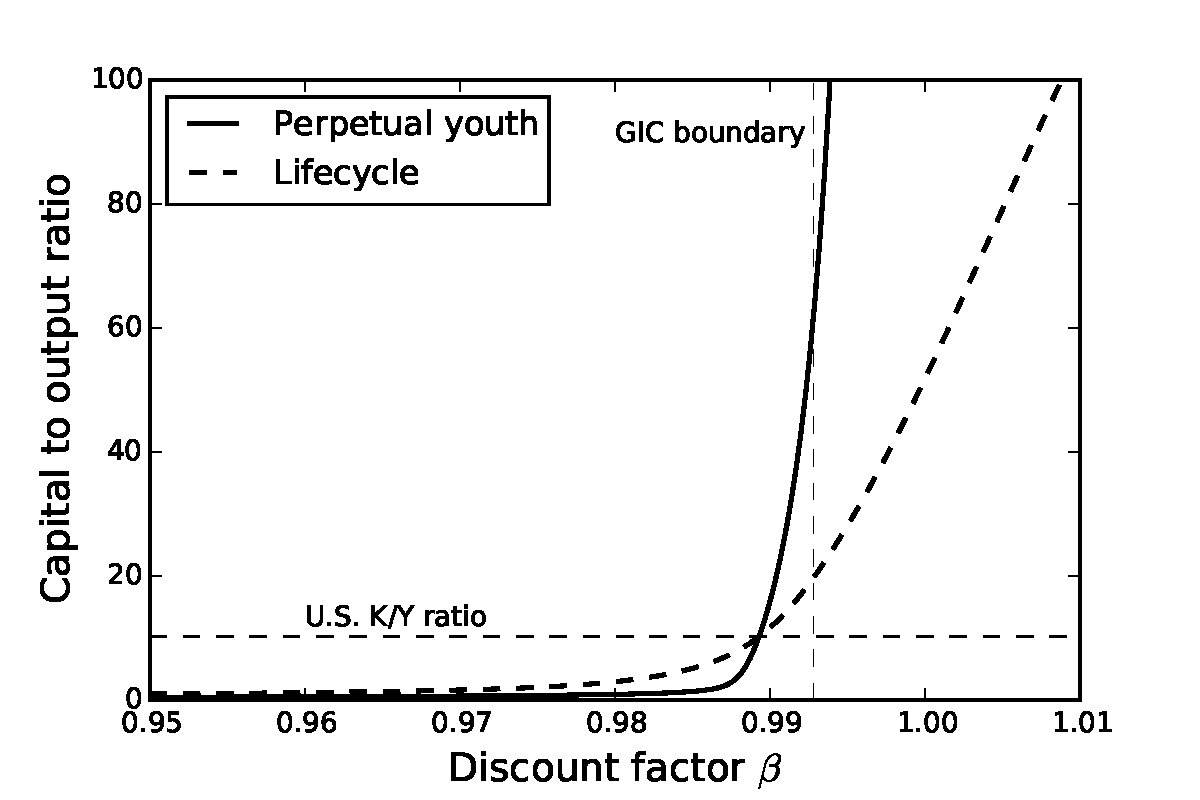
\includegraphics{./Figures/KYratioByBeta}
  \end{center}
\end{figure}

Recall that in the perpetual youth model, consumers must be sufficiently impatient in order to have a target wealth-to-income ratio: The discount factor has to meet the `Growth-Impatience Condition' \eqref{eq:GIC}. When the GIC does not hold, households accumulate wealth without bound.\footnote{Even when the GIC fails, a finite K/Y ratio for the entire economy can exist because households are finitely lived-- they die long before acquiring infinite wealth.}  As $\Discount$ increases toward the boundary of the GIC, target wealth rapidly increases toward infinity, so that small differences in $\Discount$ translate into great wealth heterogeneity (shown in Figure \ref{KYratioByBeta}).\footnote{Figure \ref{KYratioByBeta} holds $\mathsf{R}$ fixed at its steady state of 1.01, so it should be interpreted as the $K/Y$ ratio in a small open economy or for a \textit{small subset} of agents with a particular discount factor.}  In the finite-horizon life-cycle model, however, no impatience condition is required---households face an increasing mortality rate and thus will target a finite wealth ratio \textit{in a finite number of periods}, no matter how patient they are. Consequently, average wealth is a much flatter function of $\Discount$ and thus the interval needed to match the SCF data is wider.

\begin{figure}
  \caption{Distribution of Net Worth (Lorenz Curve)---Life Cycle Model}
  \label{LorenzLifecycle}
  \begin{center}
    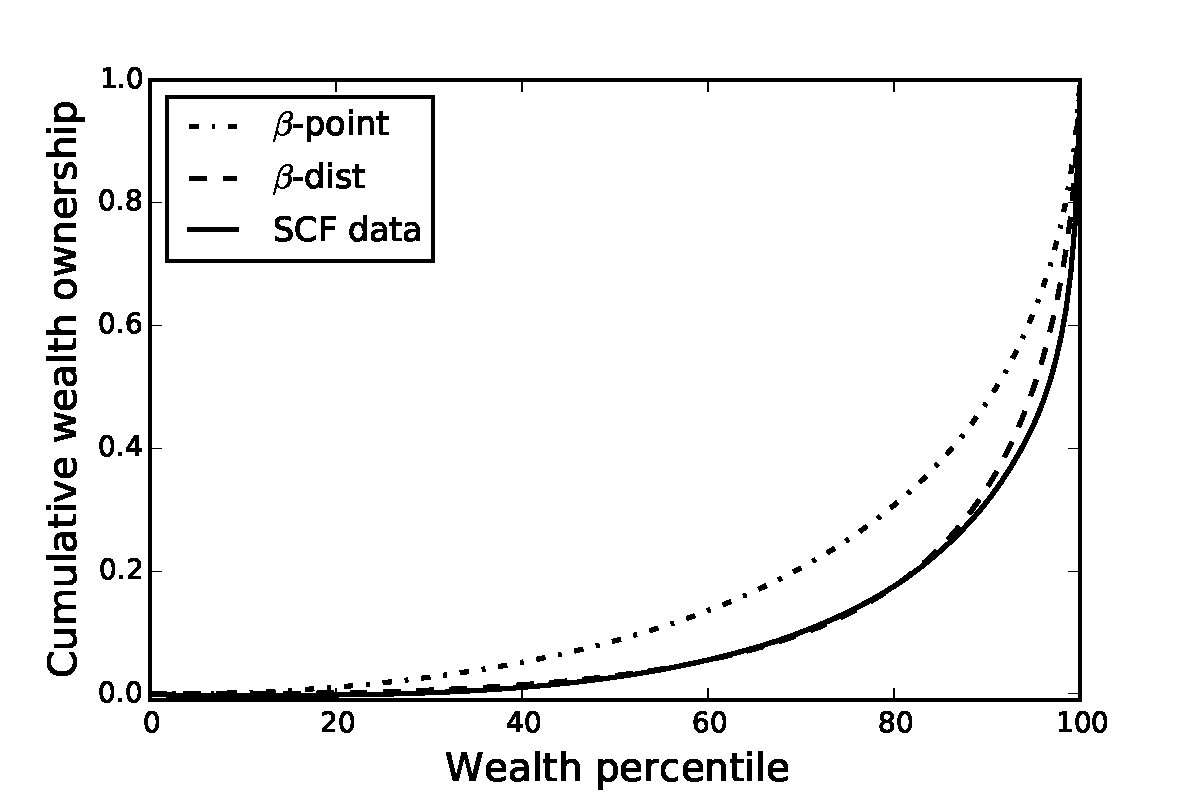
\includegraphics{./Figures/LorenzLifecycle}
  \end{center}
   \footnotesize Notes: The solid curve shows the distribution of net worth in the 2004 \emph{Survey of Consumer Finances}.
\end{figure}

The \Discount-Dist model is able to match the empirical Lorenz curve extremely well for the bottom 85\% of the wealth distribution: the average difference between simulated and actual wealth shares at the levels of interest is less than 0.4\% (Figure~\ref{LorenzLifecycle}).  Indeed, the life cycle model matches the low asset holdings of the bottom half of the population significantly better than the perpetual youth model.

However, the wealth share of the top 10\%\ in the life-cycle \Discount-Dist model is somewhat lower than in the data. In contrast, the perpetual youth model matches the Lorenz curve fairly well even in the top tail.  This also seems to be a result of the (lack of a) GIC: the lifecycle model does not have households with a very high target wealth ratio and thus cannot generate an extreme concentration of wealth in the top 1\%.  This is not a serious deficiency as the consumption function is roughly linear at higher levels of wealth and as we are concerned with the aggregate marginal propensity to consume and the MPC particularly among non-wealthy households.

The right-hand panel of Table \ref{table:MPCall} shows that, across all households, the aggregate (annual) marginal propensity to consume in both the \Discount-Point (0.16) and \Discount-Dist (0.33) models is similar to the corresponding averages in the perpetual youth model.\footnote{When the annual marginal propensity to consume is calculated by simulating the change in consumption over four quarters resulting from an unexpected \$1000 payment to each household, we find an aggregate value of 0.28, substantially the same and confirming the corresponding exercise in the perpetual youth model.}$^{,}$\footnote{Without much comment, we also present estimates of the \Discount-Dist model when matching the empirical distribution of liquid financial and retirement assets rather than net worth, along with subpopulation average MPCs for these models.  In each case, the results of the life cycle model align very well with the earlier findings in the perpetual youth setting.}  Further, the relationship between wealth-to-permanent income and the MPC is nearly identical to the pattern in the perpetual youth case, with the MPC slowly rising with lower incomes among the wealthier half of the population, and spiking rapidly among the bottom half.  However, the gradient of income to MPC is much shallower in the life-cycle model, with the wealthiest 1\% of households' MPC only 20\% less than the poorest half, rather than 50\% less in the benchmark model.  This is likely due to confounding effects from life-cycle dynamics: income-poor households are made up of both the young (who have not had time to accumulate income growth) and the retired (whose cohorts began with lower initial permanent income and have experienced the large negative wage growth from retirement).\footnote{%
  While the ratio of wealth to permanent income is a very strong determinant of the MPC, the wide distribution of household incomes allows for even wealthy households to have high MPCs.  Confirming a similar exercise in the benchmark model, we again find that among the one third of households with the highest MPCs, 51\% are in the lowest wealth quintile, 32\% are in the second wealth quintile, and 14\% are in the middle wealth quintile.  Even in a life cycle model in which wealth is highly correlated with both age and the marginal propensity to consume, there is still a significant fraction of ``wealthy hand-to-mouth'' households as found in \cite{kaplanViolanteWeidner_wealthyH2M}.}

\begin{figure}
  \caption{Aggregate Marginal Propensity to Consume by Age}
  \label{fig:MPCbyAge}
  \begin{center}
    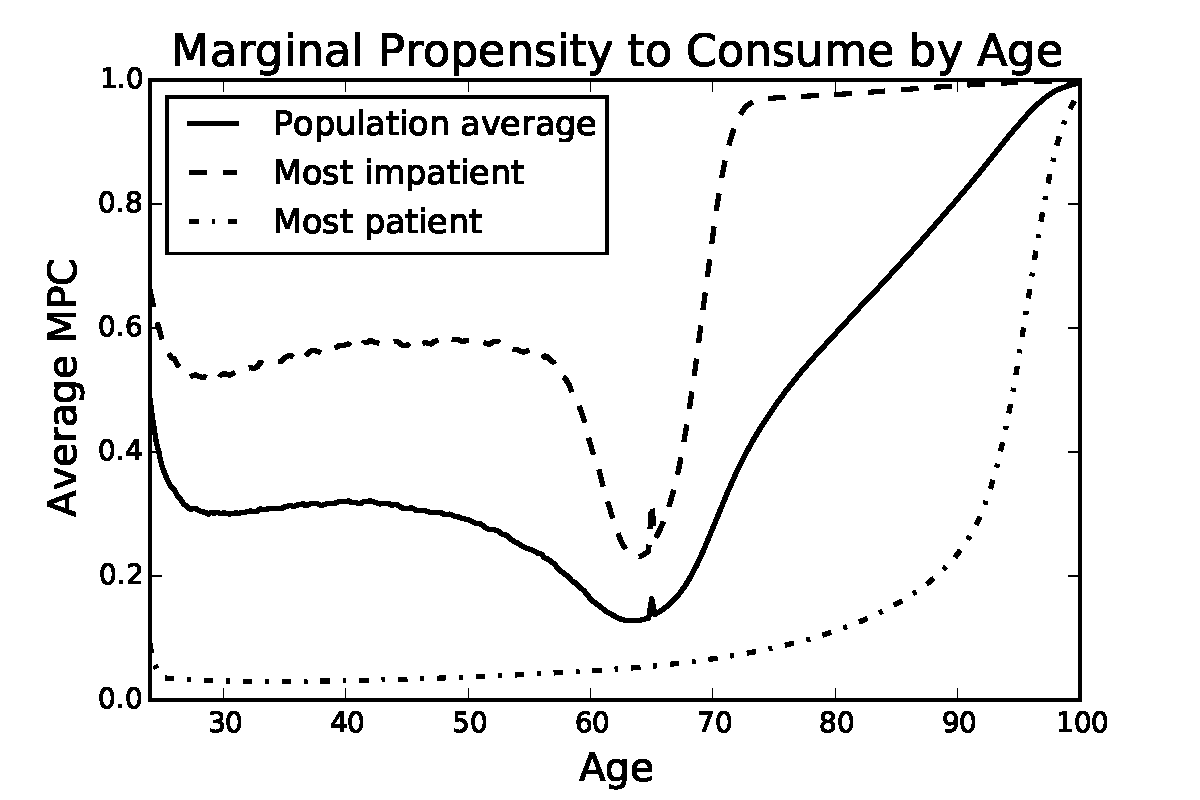
\includegraphics{./Figures/MPCbyAge}
  \end{center}
\end{figure}

Figure \ref{fig:MPCbyAge} presents the aggregate marginal propensity to consume by age for the entire population, as well as for the most patient and least patient types in the $\Discount$-Dist model.  After an initial drop as households build up a minimum buffer stock, the life cycle profile of the MPC takes an inverted U-shape for most $\Discount$ types: rising during the rapid income growth ages of 30--40 before falling as households anticipate their retirement and seek to retain assets to consume in old age.  Post retirement, the MPC steadily grows as agents experience an ever increasing mortality risk.  The most impatient households, with a quarterly discount factor of about $\beta = 0.9654$, have a significantly higher MPC throughout life as they disfavor saving---they begin saving for retirement less than ten years prior, and quickly deplete their assets if they live beyond age 75 (as evidenced by MPCs approaching 1 at these ages).  In contrast, the most patient households show an increasing marginal propensity to consume for their entire lives, though beginning from very low levels.

\section{Conclusion}\label{sec:Conclusion}

We have shown that a model with a realistic microeconomic income process and modest heterogeneity in time preference rates is able to match the observed degree of inequality in the wealth distribution.  Because many households in our model accumulate very little wealth, the aggregate marginal propensity to consume out of transitory income implied by our model, roughly 0.2--0.4 depending on the measure of wealth we ask our model to target, is consistent with most of the large estimates of the MPC reported in empirical studies. Indeed, some of the dispersion in MPC estimates from the microeconomic literature (where estimates range up to 0.75 or higher) might be explainable by the model's implication that there is no such thing as ``the'' MPC---the aggregate response to a transitory income shock should depend on details of the recipients of that shock in ways that the existing literature may not have been sensitive to (or may not have been able to measure).  If some of the experiments reported in the literature reflected shocks that were concentrated in different regions of the wealth distribution than other experiments, considerable variation in empirical MPCs would be an expected consequence of the differences in the experiments.

Additionally, our work provides researchers with an easier framework
for solving, estimating, and simulating economies with heterogeneous
agents and realistic income processes than has heretofore been
available. Although benefiting from the important insights of \citet{ksHetero},
our framework is faster and easier to solve than the KS model or many of its
descendants, and thus can be used as a convenient building block for
constructing micro-founded models for policy-relevant analysis.

\small
\input econtexBibMake

\end{document}

% Local Variables:
% mode: LaTeX
% TeX-PDF-mode: t
% TeX-parse-self: t
% TeX-auto-save: t
% End:
